%%%%%%%%%%%%%%%%%%%%%%%%%%%%%%%%%%%%%%%%%
% The Legrand Orange Book
% LaTeX Template
% Version 3.1 (February 18, 2022)
%
% This template originates from:
% https://www.LaTeXTemplates.com
%
% Authors:
% Vel (vel@latextemplates.com)
% Mathias Legrand (legrand.mathias@gmail.com)
%
% License:
% CC BY-NC-SA 4.0 (https://creativecommons.org/licenses/by-nc-sa/4.0/)
%
% Compiling this template:
% This template uses biber for its bibliography and makeindex for its index.
% When you first open the template, compile it from the command line with the 
% commands below to make sure your LaTeX distribution is configured correctly:
%
% 1) pdflatex main
% 2) makeindex main.idx -s indexstyle.ist
% 3) biber main
% 4) pdflatex main x 2
%
% After this, when you wish to update the bibliography/index use the appropriate
% command above and make sure to compile with pdflatex several times 
% afterwards to propagate your changes to the document.
%
%%%%%%%%%%%%%%%%%%%%%%%%%%%%%%%%%%%%%%%%%

%----------------------------------------------------------------------------------------
%	PACKAGES AND OTHER DOCUMENT CONFIGURATIONS
%----------------------------------------------------------------------------------------

\documentclass[
	11pt, % Default font size, select one of 10pt, 11pt or 12pt
	fleqn, % Left align equations
	a4paper, % Paper size, use either 'a4paper' for A4 size or 'letterpaper' for US letter size
]{LegrandOrangeBook}

\usepackage[utf8]{inputenc}
\usepackage[italian]{babel}
\usepackage{amssymb}
\usepackage{amsmath}
\usepackage{subfig}

\DeclareMathOperator{\der}{d}

\hypersetup{
	pdftitle={Astroparticelle}, % Title field
	pdfauthor={Matteo Brini}, % Author field
	pdfsubject={Fisica}, % Subject field
}

\addbibresource{astro.bib} % Bibliography file

\chapterimage{img/spaceimg.jpg}
\definecolor{ocre}{RGB}{243, 102, 25} % Define the color used for highlighting throughout the book

%\chapterimage{orange1.jpg} % Chapter heading image
\chapterspaceabove{6.5cm} % Default whitespace from the top of the page to the chapter title on chapter pages
\chapterspacebelow{6.75cm} % Default amount of vertical whitespace from the top margin to the start of the text on chapter pages

%----------------------------------------------------------------------------------------

\begin{document}

%----------------------------------------------------------------------------------------
%	TITLE PAGE
%----------------------------------------------------------------------------------------

\titlepage % Output the title page
	{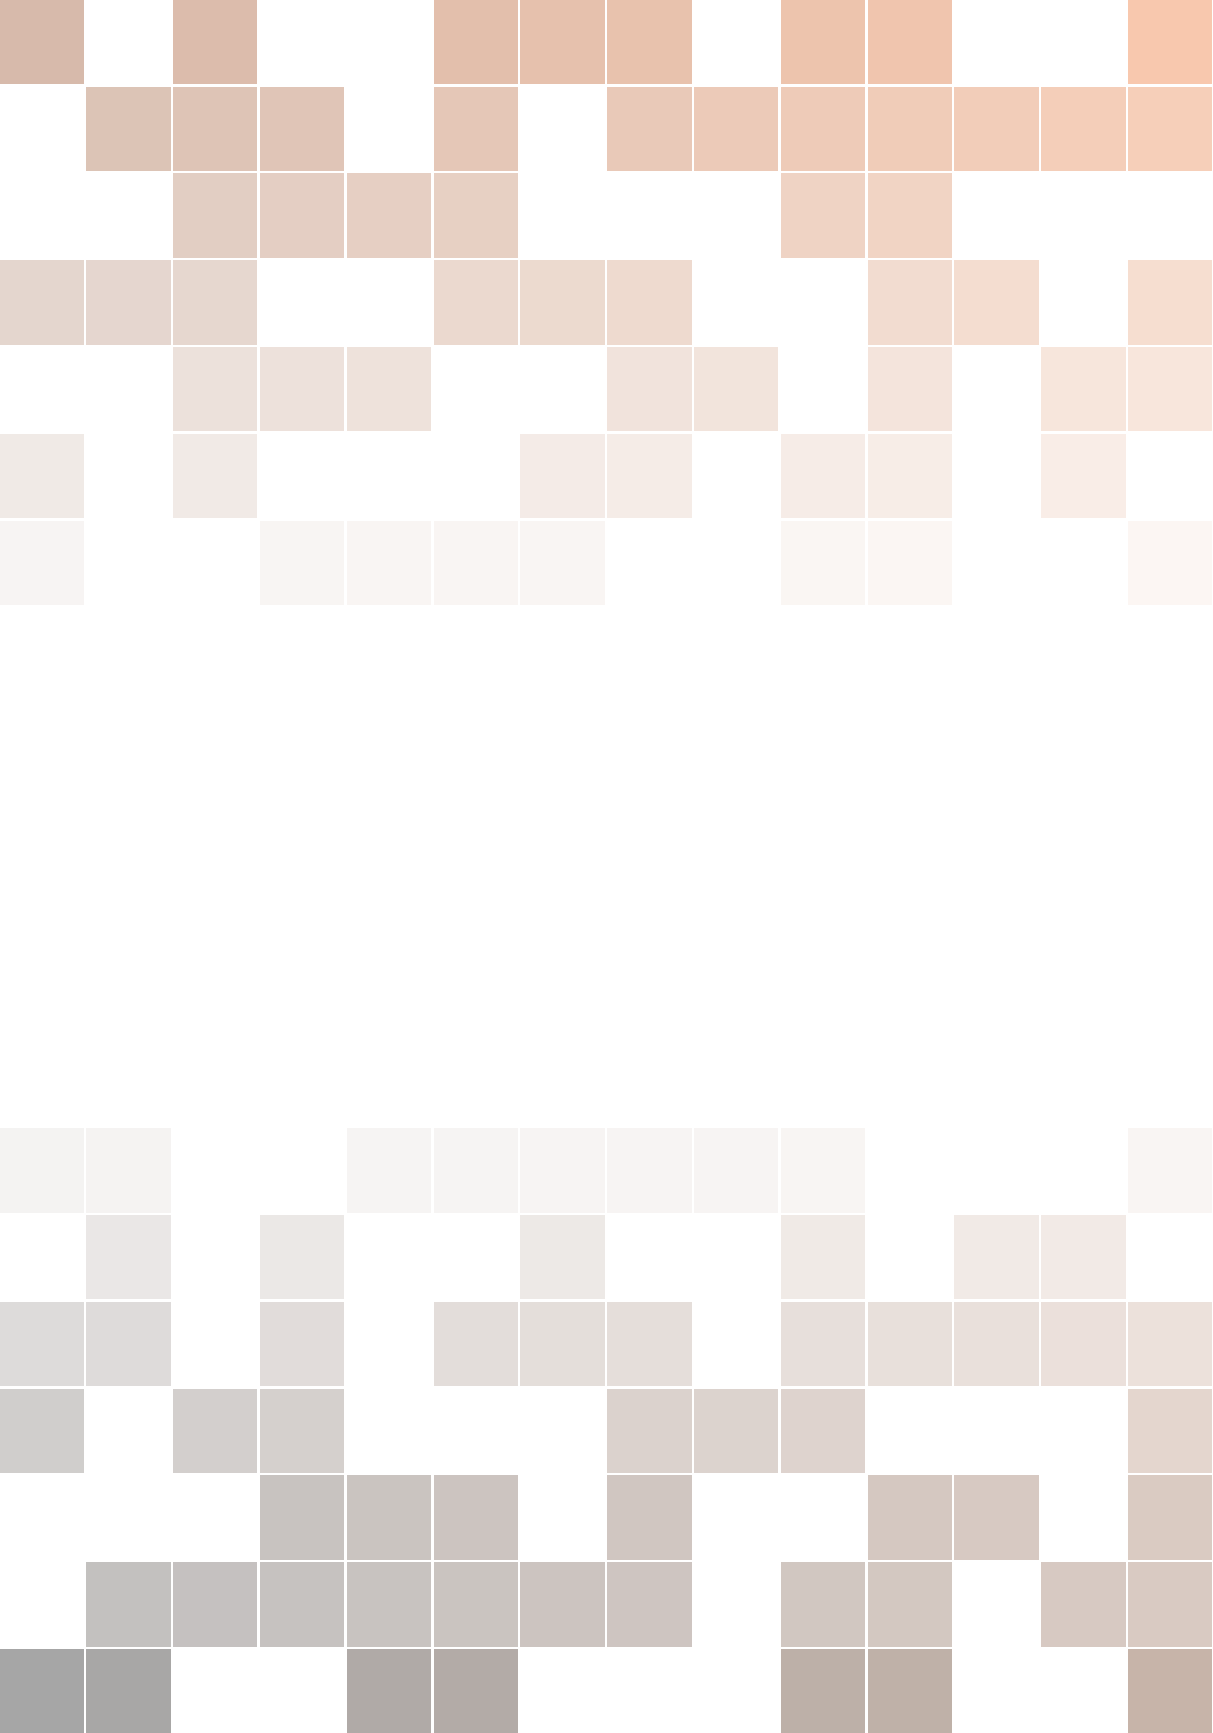
\includegraphics[width=\paperwidth]{img/background.pdf}} % Code to output the background image, which should be the same dimensions as the paper to fill the page entirely; leave empty for no background image
	{ % Title(s) and author(s)
		\centering\sffamily % Font styling
		{\Huge\bfseries Lezioni di Astroparticelle\par} % Book title
		\vspace{16pt} % Vertical whitespace
		{\LARGE Appunti del corso A.A. 2022-2023\par} % Subtitle
		\vspace{24pt} % Vertical whitespace
		{\huge\bfseries Matteo Brini\par} % Author name
	}

%----------------------------------------------------------------------------------------
%	COPYRIGHT PAGE
%----------------------------------------------------------------------------------------

\thispagestyle{empty} % Suppress headers and footers on this page

~\vfill % Push the text down to the bottom of the page

\noindent Copyright \copyright\ 2023 Matteo Brini\\ % Copyright notice

\noindent \textsc{\href{https://github.com/brinus}{github.com}}\\ % URL

\noindent Questo libro si pone la finalià di contenere le informazioni \textit{necessarie e sufficienti} per il superamento dell'esame di Astroparticelle. Il contenuto di questo libro è il frutto della ristesura delle lezioni frontali tenute dal Professor A. Baldini durante l'anno accademico 2022-2023, nonchè degli approfondimenti di diversi libri di testo consultati durante questa stesura. Lo stile adottato per il libro è stato ideato da \href{https://www.latextemplates.com/template/legrand-orange-book}{Mathias Legrand}. Per ogni problema o informazione si contatti \href{mailto:brinimatte@gmail.com}{brinimatteo@gmail.com}.\\
\noindent \textit{Prima stampa, Giugno 2023} % Printing/edition date

%----------------------------------------------------------------------------------------
%	TABLE OF CONTENTS
%----------------------------------------------------------------------------------------

\pagestyle{empty} % Disable headers and footers for the following pages

\tableofcontents % Output the table of contents

\pagestyle{fancy} % Enable default headers and footers again

\cleardoublepage % Start the following content on a new page

\part{Prima Parte}
\chapterimage{img/SuperKK.jpg} % Chapter heading image
\chapterspaceabove{6.75cm} % Whitespace from the top of the page to the chapter title on chapter pages
\chapterspacebelow{7.25cm} % Amount of vertical whitespace from the top margin to the start of the text on chapter pages

%------------------------------------------------

\chapter{Introduzione}\index{Introduzione}

In questo capitolo vengono introdotti i contenuti e le finalità del corso. Vengono inoltre introdotti i concetti base del corso.


\section{Informazioni sul corso e finalità}\index{Finalità del corso}

Si riporta dalla pagina \href{https://elearning.df.unipi.it/course/view.php?id=237}{e-learning} del corso la finalità di questo esame:
\begin{quote}
    Nella prima parte del corso lo studente dovrà acquisire una certa conoscenza delle principali caratteristiche dei raggi cosmici e dei metodi utilizzati per la loro rilevazione, conoscenze sui recenti sviluppi nelle misure e rivelazione di neutrini dal sole, conoscenza molto elementare della relatività generale e di come derivare le equazioni di Friedmann-Lemaitre, conoscenza di base dei modelli cosmologici standard, dei suoi limiti e dei possibili candidati alla materia oscura, conoscenza dei metodi di rivelazione sperimentale diretta e indiretta di candidati materia oscura. 
    Nella seconda parte del corso si richiede allo studente di acquisire una conoscenza di base della teoria e della rivelazione delle onde gravitazionali.
\end{quote}

\section{Introduzione storica}\index{Introduzione!Introduzione storica}

Cominciamo studiando la storia dei raggi cosmici. Le prime ipotesi risalgono a Charles Coulomb, che nel 1785 osservò con un elettroscopio a foglie che questo si scaricava spontaneamente nel tempo: ciò portò all'ipotizzazione di una carica presente nell'aria circostante. Studi successivi di Hess e Kolhörster misurano (con l'uso di palloni aerostatici) l'aumento della capacità ionizzante di questo \emph{qualche cosa} con l'aumentare dell'altitudine. Il fisico statunitense Millikan confermò con i suoi studi l'orignie extraterrestre di queste particelle e decise di chiamarle \emph{raggi cosmici}. 

I raggi cosmici hanno dato vita alla fisica delle particelle elementari, si ricordi ad esempio nel 1930 la scoperta del positrone da parte di Anderson, la scoperta dei mesoni $\pi^\pm$ e $\textup{K}^\pm$ nel 1947. Negli anni '50 vengono costruiti i primi acceleratori di particelle, gli acceleratori odierni raggiungono energie nel centro di massa di $10^{13}\,\textup{eV}$.

\begin{figure}[H]
    \centering
    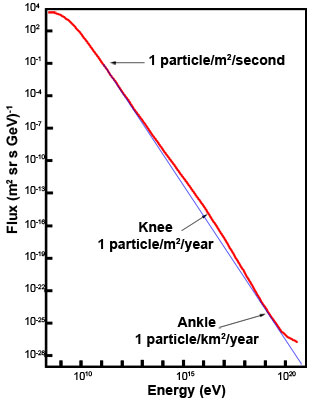
\includegraphics[width=0.35\textwidth]{img/cosmicrayenergies1.jpg}
    \caption{Spettro in energia dei raggi cosmici. Si osservino in particolare i due gomiti dello spettro.}    
    \label{img:cosmicrays}
\end{figure}

\begin{example}
    Proviamo adesso a confrontare le energie dei protoni provenienti dallo spazio che urtano su altri protoni fermi, con le energie dei protoni di LHC. In questo esempio verrà assunto $c = 1$. Supponiamo due protoni che si scontrano, viaggiando in direzione opposta lungo l'asse $\hat{z}$:
    \begin{gather*}
        p_1^\mu = (E^*, 0, 0, \vec{p}), \\
        p_2^\mu = (E^*, 0, 0,  -\vec{p}).
    \end{gather*}
    Dobbiamo confrontare questo caso con quello in cui abbiamo un protone fermo ed uno diretto verso il primo con una certa quantità di moto:
    \begin{gather*}
        p_1'^\mu = (m_\textup{p}, 0, 0, 0), \\
        p_2'^\mu = (E, 0, 0, \vec{p}').
    \end{gather*}
    Sommando semplicemente i primi due 4-vettori, otteniamo che per i protoni nel caso di LHC vale
    \begin{equation*}
        2E^* = E_\textup{cm} \simeq 10^13\,\textup{eV}.
    \end{equation*}
    Per i protoni nel secondo caso abbiamo invece
    \begin{equation*}
        \begin{split}
            (p_1'^\mu + p_2'^\mu)^2 & = (p_1'^\mu)^2 + (p_2'^\mu)^2 + p_1'^\mu \cdot p_2'_\mu \\
                                    & \simeq 2Em_\textup{p} \\
                                    & \simeq (10^{13}\,\textup{eV})^2,
        \end{split}
    \end{equation*}
    dove l'ultimo passaggio viene assunto valido dal momento in cui si vuole confrontare l'energia dei due processi, abbiamo inoltre trascurato un termine proporzionale a $m_\textup{p}^2$. Si ricava dunque
    \begin{equation*}
        E \simeq \frac{(10^{13}\,\textup{eV})^2}{2m_\textup{p}} \simeq 5 \times 10^{16}\,\textup{eV}.
    \end{equation*}
    Questa è l'energia che deve avere un protone proveniente dallo spazio che, urtando su un protone fermo presente nell'atmosfera, dà un'energia nel centro di massa pari a quella di LHC. Confrontando questa informazione con il grafico in figura Fig.(\ref{img:cosmicrays}) vediamo che gli esperimenti condotti ad LHC ci permettono di concludere osservazioni su particelle provenienti da raggi cosmici che corrispondono ad energie nell'intorno del primo ginocchio del grafico.
\end{example}

Con il progredire delle misure fatte sugli sciami cosmici, si sono osservati anche gli andamenti dei flussi in funzione del numero atomico $Z$: in particolare si è osservato come la composizione dei raggi cosmici comprendesse tutti i nuclei fino al Fe per poi fermarsi. In figura Fig.(\ref{img:cosmicZ}) si riporta l'andamento di tali flussi, in tabella Tab.(\ref{tab:cosmicZ}) si riporta in particolare il flusso relativo a quello di Fig.(\ref{img:cosmicrays}).

\begin{figure}[H]
    \centering
    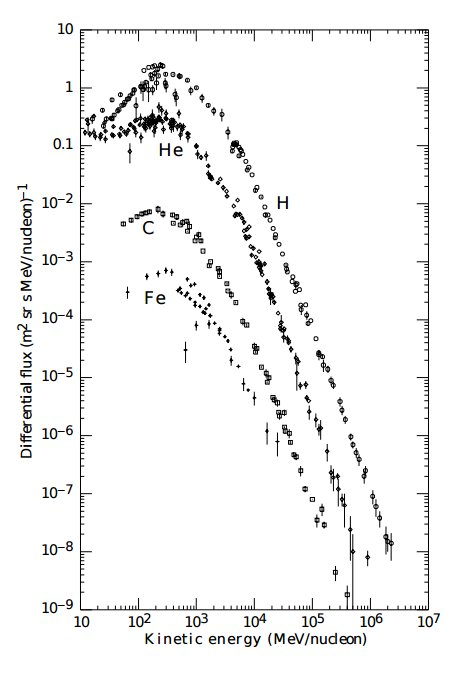
\includegraphics[width=0.4\textwidth]{img/cosmicrayZ.jpg}
    \caption{Andamento dei flussi per diversi nuclei.}  
    \label{img:cosmicZ}  
\end{figure}

\begin{table}[H]
    \centering
    \begin{tabular}{lll}
        \toprule
        \textbf{Z} & \textbf{Elemento} & \textbf{Flusso relativo} \\
        \midrule
        1          & H                 & 540                      \\
        2          & He                & 26                       \\
        3-5        & Li-B              & 0.40                     \\
        6-8        & C-O               & 2.20                     \\
        9-10       & F-Ne              & 0.30                     \\
        \bottomrule
    \end{tabular}
    \caption{Valori di flusso relativo per i nuclei che compongono i raggi cosmici, in rapporto al flusso totale misurato.}
    \label{tab:cosmicZ}
\end{table}

Inoltre sappiamo che:
\begin{itemize}
    \item il flusso di elettroni è circa due ordini di grandezza inferiore a quello dei protoni,
    \item il flusso di positroni è circa $1/20$ di quello degli elettroni,
    \item il flusso di antiprotoni è circa $10^{-4}$ di quello dei protoni.
\end{itemize}
Osservazioni negli anni del flusso di protoni mostrano che la componente a bassa energia nello spettro del flusso di protoni dallo spazio cambia nel tempo: questo è presumibilmente legato all'attività magnetica solare. Non ci sono variazioni nella parte di flusso ad alta energia ($\gtrsim 1\,\textup{GeV}$).

\section{Richiami di perdita di energia delle particelle nella materia}\index{Perdita di energia nella materia}

L'interazione fra particelle e la materia viene classificata sulla base della carica e della massa (al solito, i neutrini
fanno storia a sè). Quando parliamo di particelle pesanti cariche (tipicamente adroni), vogliamo studiare il loro passaggio nella materia: nelle condizioni più comuni ($m \gg m_\textup{e}$, piccolo impulso trasferito, elettrone atomico libero e in quiete) possiamo parlare di ionizzazione del materiale. La grandezza di interesse è $-\der E / \der x$, questa segue la nota formula di Bethe-Block:
\begin{equation*}
    -\frac{\der E}{\der x} = 2\pi N_\textup{A} r_\textup{e}^2 m_\textup{e} c^2 \frac{Z}{A} \frac{^2}{\beta} \biggl[ \ln \frac{2m_\textup{e}c^2 \gamma^2 \beta^2 W_\textup{max}}{I^2} 2\beta^2 - \delta - 2\frac{C}{Z}\biggr].
\end{equation*}
Questa formula descrive la perdita di energia per ionizzazione del mezzo in funzione della \emph{lunghezza ridotta} $x = L\rho$, essendo $\rho$ la densità del mezzo. La perdita di energia viene chiamata anche \emph{stopping power} del mezzo attraversato.

Gli elettroni non perdono energia nella stessa maniera delle altre particelle. Ci sono due meccanismi principali con cui gli elettroni perdono energia:
\begin{itemize}
    \item Collisione atomiche (ionizzazione), in questo caso vale il seguente andamento:
    \begin{equation*}
        -\frac{\der E}{\der x} \biggr|_\textup{Coll} \varpropto Z \ln E_0,
    \end{equation*}
    \item Bremmtrahlung, in questo caso vengono emessi fotoni nel campo di un nucleo
    \begin{equation*}
        -\frac{\der E}{\der x} \biggr|_\textup{Brem} \varpropto Z^2 E_0.
    \end{equation*}
\end{itemize}
Ciascuno dei due processi domina sull'altro a diverse scale di energia.
\begin{definition}[Energia critica]
    L'energia a cui i due processi si equivalgono viene definita con il nome di \emph{energia critica}, empiricamente è descritta dalla seguente formula:
    \begin{equation*}
        E_\textup{C} \approx \frac{800\,\textup{MeV}}{Z + 1}.
    \end{equation*}
    Al di sopra dell'energia critica, la perdita di energia dovuta al processo di Bremmstrahlung è maggiore di quella per ionizzazione.
\end{definition}

I fotoni hanno vari meccanismi di perdita di energia, i tre più importanti sono i seguenti:
\begin{itemize}
    \item effetto fotoelettrico a basse energie ($\lesssim 1\,\textup{keV}$), $\sigma \varpropto Z^5$,
    \item scattering Compton a energie intermedie ($\simeq 1\,\textup{MeV}$), $\sigma \varpropto Z$,
    \item produzione di coppie ad alte energie ($E_\gamma \geqslant 2m_\textup{e}c^2$, dominante per $E > 20\,\textup{MeV}$), $\sigma \varpropto Z(Z+1)$.
\end{itemize}

\subsection*{Calorimetria}

Quando un fotone o un elettrone con elevata energia urta contro un materiale, si dà orignie ad uno \emph{sciame elettromagnetico} (che differisce da quello \emph{adronico}, ne parleremo più avanti). I processi dominanti sono quelli di Bremmstrahlung e produzione di coppie, gli elettroni e fotoni urtando con i centri scatteranti del materiale attraversato originano altri elettroni e fotoni secondari, il processo si può ripetere un certo numero di volte. Volendo caratterizzare l'intensità dello sciame possiamo scrivere:
\begin{equation}
    I = I_0e^{-x/X_0}   \begin{cases}
                            e^- N \rightarrow e^- N \gamma, \quad X_0 \\
                            \gamma N \rightarrow N e^+ e^-, \quad \frac{9}{7}X_0
                        \end{cases}. 
    \label{eq:intensita_X0}      
\end{equation}
\begin{definition}[Lunghezza di radiazione]
    Si definisce \emph{lunghezza di radiazione} la quantità $X_0$, definita come la distanza media (in cm) che un elettrone deve percorrere nel materiale per ridurre la sua energia di un fattore $1/e$ solo per effetto della radiazione. Per la lunghezza di radiazione vale la seguente formula:
    \begin{equation*}
        \frac{1}{X_0} = 4\alpha r_\textup{e}^2\frac{N_\textup{A}}{A} \bigl\{ Z^2\left[L_\textup{rad} - f(Z)\right] + ZL_\textup{rad}'\bigr\}. 
    \end{equation*}
    Da Eq.(\ref{eq:intensita_X0}) si osservi che la lunghezza in cui i fotoni compiono una produzione di coppia equivale a circa i $\frac{9}{7}X_0$, questa lunghezza è anche chiamata \emph{cammino libero medio} per il processo di produzione di coppie.
\end{definition}

Possiamo modellizzare l'evoluzione di uno sciame elettromagnetico osservando che circa ogni $X_0$ vengono prodotte due nuove particelle a partire da una singola particella, inoltre il processo si ripete fino a quando $E > E_\textup{c}$, in particolare dopo $nX_0$ lunghezza ho $2^n$ particelle:
\begin{gather*}
    E_\textup{p}   = \frac{E_0}{2^n},\\
    E_\textup{c}   = \frac{E_0}{2^{n_\textup{max}}} = E_{\textup{n}_\textup{max}},\\
    n_\textup{max} = \ln \frac{E_0}{E_\textup{c}} \frac{1}{\ln 2}.
\end{gather*}
Secondo il modello precendente, l'energia non viene rilasciata prima di $n_\textup{max}$, dove invece viene rilasciata tutta insieme. Chiaramente lo sviluppo reale è più complesso di così ma qualitativamente si può dire che:
\begin{itemize}
    \item l'andamento iniziale della curva ha un andamento molto veloce dovuto alla \emph{moltiplicazione} delle particelle nello sciame,
    \item si arriva ad un massimo quando le coppie secondarie hanno energia $E_\textup{c}$,
    \item dopo quel punto non c'è più moltiplicazione nello sciame e c'è una discesa lenta,
    \item le dimensioni longitudinali dello sciame crescono logaritmicamente con $E_0$.
\end{itemize}

Quando parliamo di sciami adronici invece, è bene ricordare quali sono i due meccanismi principali di perdita di energia:
\begin{itemize}
    \item interazioni degli adroni con gli elettroni del materiale, dunque perdita di energia per ionizzazione,
    \item interazione degli adroni con il nucleo atomico, dunque urto anelastico con il nucleo con conseguente produzione di adroni leggeri ($\pi^0$ e $\pi^\pm$).
\end{itemize}
Ricordiamo adesso alcune formule utili che ci permettono di schematizzare la \emph{lunghezza di interazione adronica}:
\begin{gather*}
    r_\textup{N} \sim r_\textup{f} \times \sqrt[3]{A}, \\
    \sigma_\textup{N} \varpropto r_\textup{N}^2 \varpropto A^{\frac{2}{3}}, \\
    \lambda_\textup{I} = \frac{1}{\rho_\textup{B}\sigma} \varpropto A^{\frac{1}{3}} \varpropto r_\textup{N}.
\end{gather*}
Gli adroni, in quanto tali, danno vita a sciami che differiscono per alcune caratteristiche da quelli elettromagnetici:
\begin{itemize}
    \item le dimensioni longitudinali e trasversali sono diverse,
    \item la componente \textit{em} prodotta dal decadimneto dei $\pi^0$ è soggetta a forti fluttuazioni, ma in generale varia con l'energia della particella iniziale.
    \item c'è una certa frazione di energia invisibile, dovuta alla presenza di $\nu$ e $\mu$,
    \item i neutroni prodotti durante l'urto anelastico vengono termalizzati e riassorbiti con un certo ritardo.
\end{itemize}
Lo strumento per eccellenza per campionare la perdita di energia (per ionizzazione) nella materia è il \emph{calorimetro}. Questo può essere costruito in vari modi: si classificano per scopo (elettromagnetici o adronici), materiale (gas, di scintillazione, cristalli, liquidi...), composizione (omogenei o a \emph{sampling}) e modalità di lettura (compensazione, double-readout, PFA).

\subsection*{Effetto Cherenkov}

Una particella carica che si muove in un mezzo dielettrico emette onde elettromagnetiche che si propagano a velocità $c/n$, con $n$ indice di rifrazione del mezzo. Se la particella che si propaga nel mezzo ha velocità maggiore di quella nella luce nello stesso mezzo si ha una emissione di un fronte d'onda coerente con un determinato angolo di inclinazione rispetto alla direzione di propagazione della particella. 

\begin{figure}[H]  
    \centering
    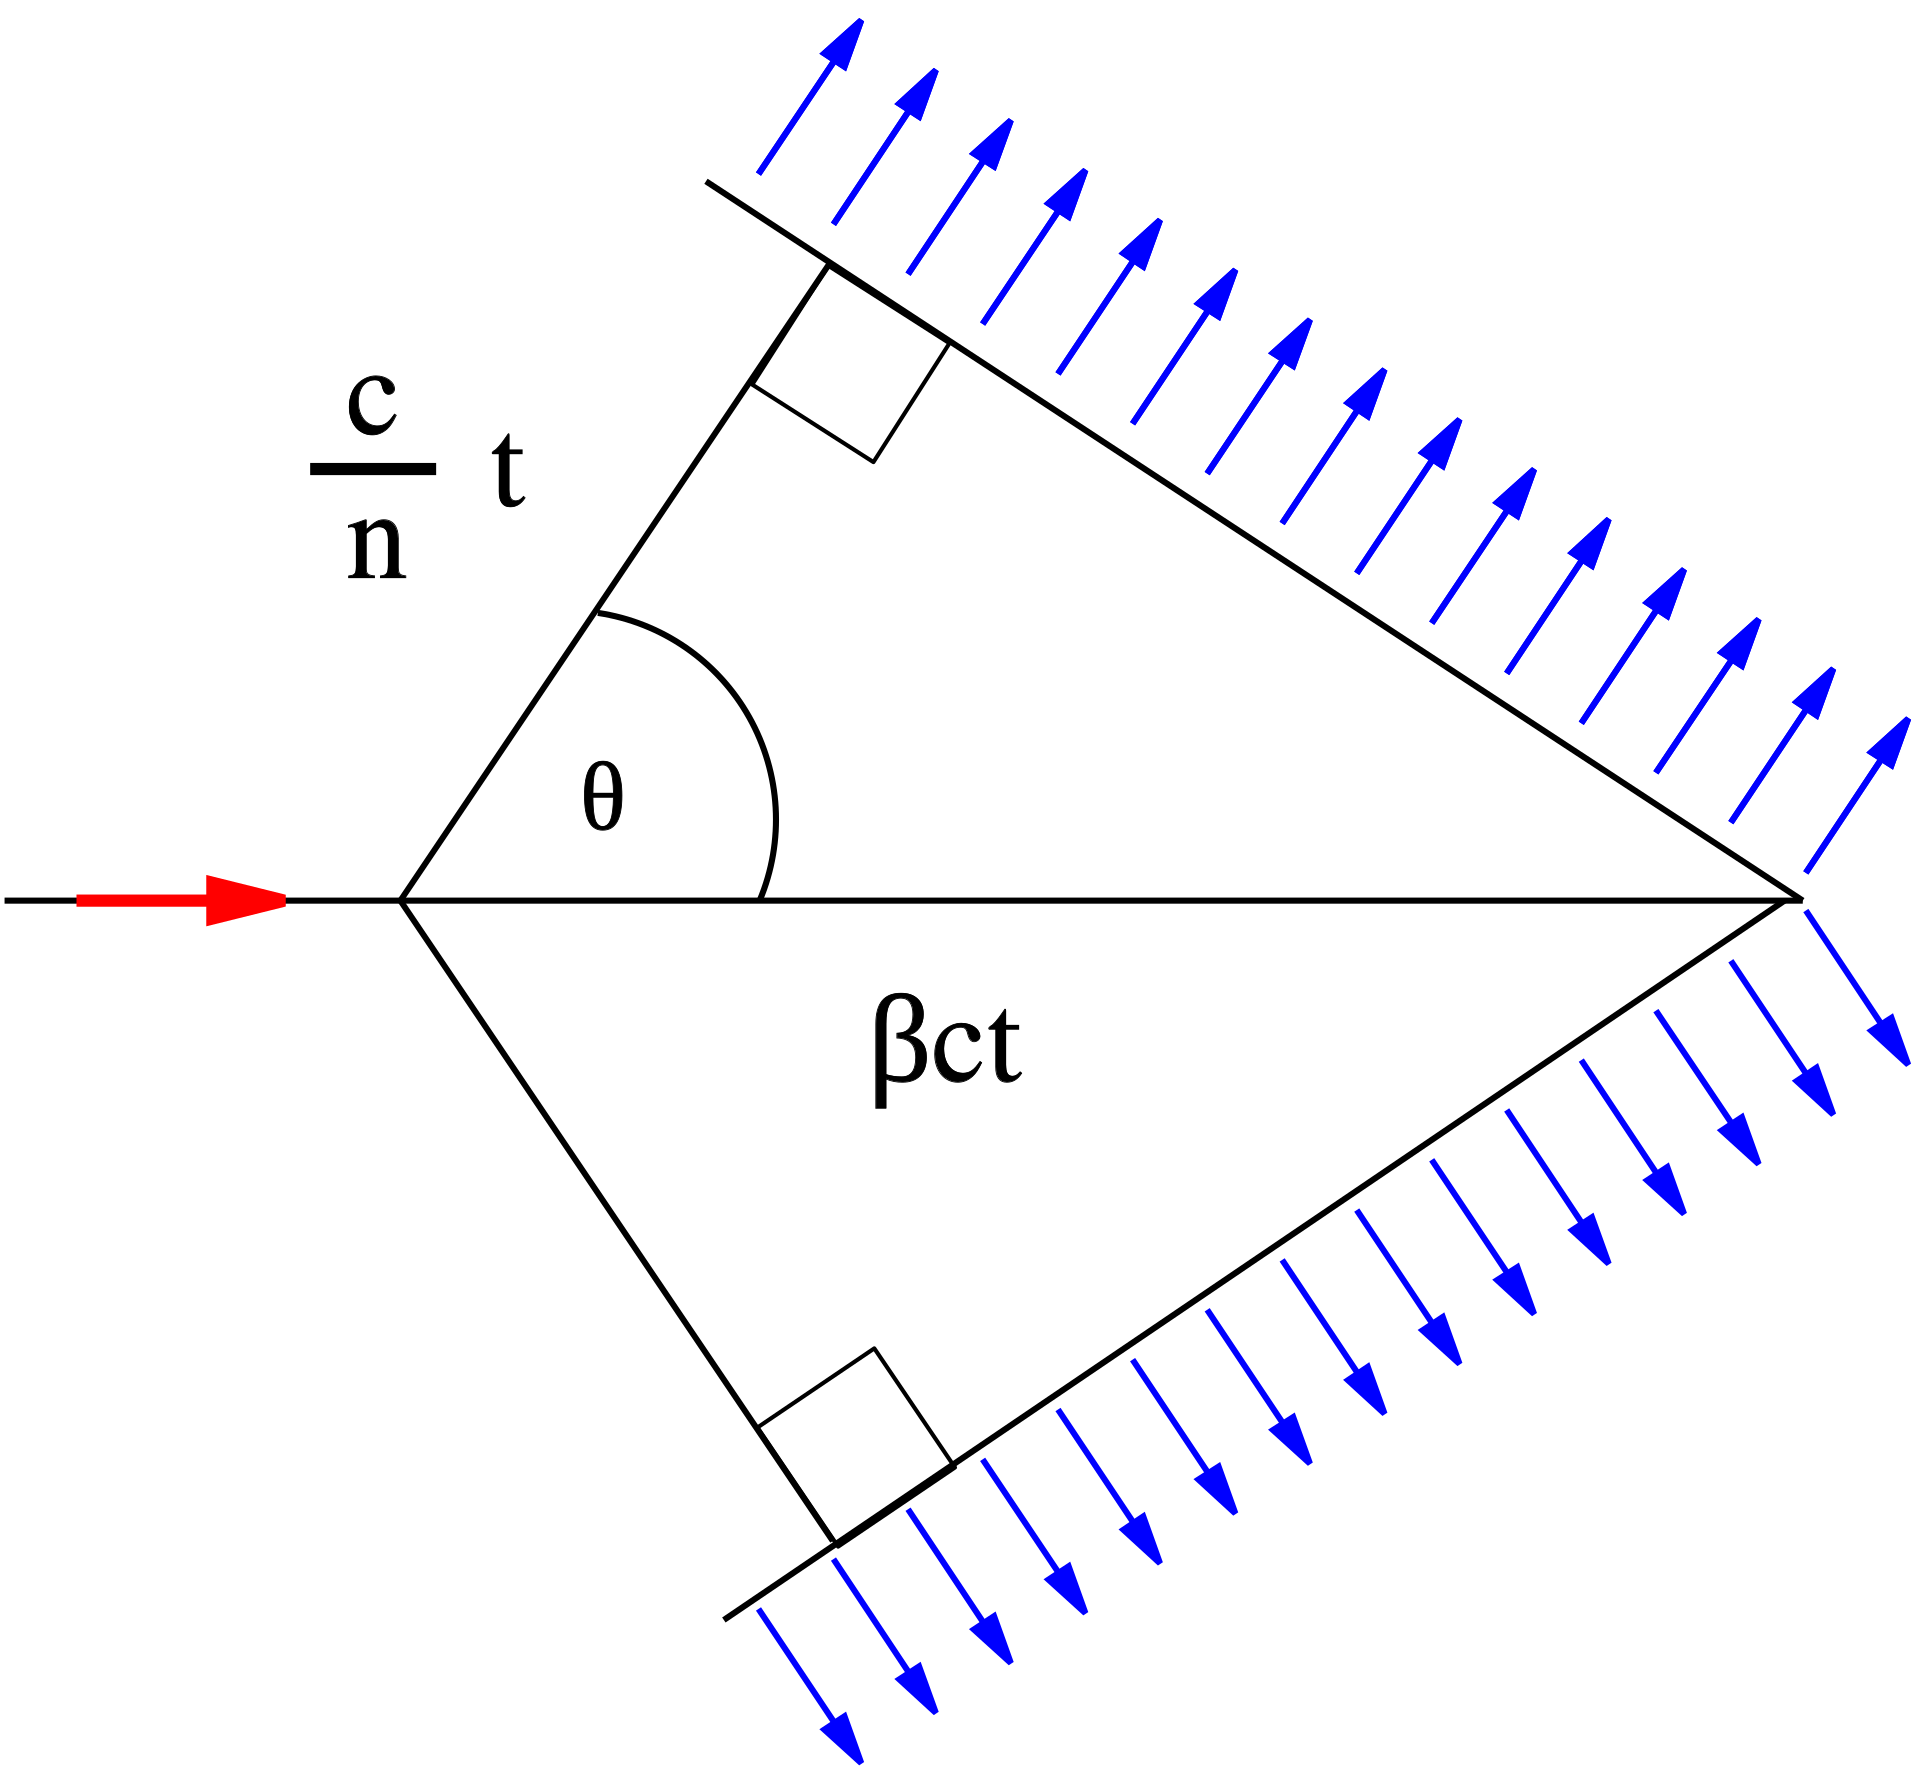
\includegraphics[width=0.4\textwidth]{img/cherenkov_effect.png}
    \caption{Schematizzazione geometrica dell'effetto Cherenkov. In rosso si indica la direzione di propagazione della particella, in blu la direzione del fronte d'onda.}
    \label{img:cherenkov_effect}
\end{figure}
Come si evince dalla figura Fig.(\ref{img:cherenkov_effect}), possiamo scrivere la relazione tra l'angolo $\theta$ e la velocità $\beta$ della particella:
\begin{equation*}
    \cos \theta = \frac{1}{n\beta}.
\end{equation*}
Dall'informazione sul cono di luce emesso possiamo inferire informazioni sulla direzione della particella. Un altro punto fondamentale dell'effetto Cherenkov è che fa da soglia, in quanto l'emissione avviene solo se vale $\beta > 1/n$. Combinando questa informazione con quella della massa della particella posso stimare l'energia della particella (usando la nota relazione $E = m\gamma c^2$).
\chapterimage{img/SuperKK.jpg} % Chapter heading image
\chapterspaceabove{6.75cm} % Whitespace from the top of the page to the chapter title on chapter pages
\chapterspacebelow{7.25cm} % Amount of vertical whitespace from the top margin to the start of the text on chapter pages

%------------------------------------------------

\chapter{Raggi cosmici}\index{Raggi cosmici}

In questo capitolo si affronta il primo argomento trattato dal corso: i raggi cosmici. Lo scopo è quello di dare informazioni sui vari esperimenti condotti a terra sulla misurazione di proprietà importanti degli sciami originati da particelle provenienti dallo spazio, nonchè studiare alcuni tra i principali meccanismi di accelerazione di queste particelle. L'obiettivo principale è quello di comprendere e modellizzare l'andamento dello spettro in energia in Fig.(\ref{img:cosmicrays}).

\section{Rivelazione di raggi cosmici}

Come si misurano i raggi cosmici? Non esiste una risposta esaustiva, ovviamente dipende da dove vengono rivelati.
\begin{itemize}
    \item Misurazioni fuori dall'atmosfera:
    \begin{itemize}
        \item assenza di atmosfera,
        \item dimensioni limitate per problemi logistici e di costo.
    \end{itemize}
    \item Con palloni aerostatici:
    \begin{itemize}
        \item basso costo, atmosfera residua limitata,
        \item brevi periodi di vita ($\sim$ settimane).
    \end{itemize}
    \item Dal suolo terrestre:
    \begin{itemize}
        \item larghe aree coperte (ordine del km$^2$),
        \item schermo dell'atmosfera, si osservano i prodotti secondari.
    \end{itemize}
    \item Dal sottosuolo:
    \begin{itemize}
        \item grossi volumi, adatti per fisica dei neutrini,
        \item difficoltà tecniche per luogo e dimensioni.
    \end{itemize}
\end{itemize}
Quando si progetta un esperimento che vuole rivelare particelle provenienti dalle regioni dello spettro a maggior energia, facendo riferimento a Fig.(\ref{img:cosmicrays}), bisogna tener di conto del flusso di tali particelle: sarebbe ad esempio impensabile di condurre dallo spazio un esperimento per la misura di particelle con energie dell'ordine di $10^{18}\,\textup{eV}$, essendo che siamo in grado di mandare in orbita strumentazioni con dimensioni ridotte (si noti dalla figura che in questo caso stiamo cercando di misurare flussi dell'ordine di $1\,\textup{evt}/\textup{y}\cdot\textup{km}^2$). Dobbiamo dunque, in questo caso, accettare il fatto di fare la misura da terra e convivere con la presenza di particelle secondarie.

Quando un nucleo proveniente dallo spazio incontra l'atmosfera terrestre infatti dà luogo ad uno sciame. Come visto in precedenza ci sono alcuni processi importanti, due esempi da tenere bene a mente sono i seguenti:
\begin{gather*}
    \pi^{+} \rightarrow \mu^+ + \nu_\mu, \\
    \mu^+   \rightarrow e^+ + \bar{\nu}_\mu + \nu_e,
\end{gather*}
e ovviamente i rispettivi processi con il coniugato di carica. Dunque possiamo assumere che l'atmosfera in questo si comporta proprio come un calorimetro. Il massimo di uno sciame, come già accennato in precedenza, si ha ad una profondità proporzionale al logaritmo dell'energia della particella incidente. La maggior parte degli esperimenti condotti dal suolo terrestre si trova su altopiani, con lo scopo di rivelare il maggior numero di particelle provenienti da uno sciame e di ridurre le fluttuazioni statistiche dovute alla frazione elettromagnetica dello sciame.

\section{Esperimenti sui raggi cosmici}\index{Raggi cosmici!Esperimenti}

Gli esperimenti che si svolgono sul suolo, sono posti alla massima altezza possibile (ordine di $2-3\,\textup{km}$), alcuni siti di esempio sono in Argentina e Cile. Questi esperimenti mappano un terreno vasto con un certo numero di rivelatori, misurando informazioni di spazio (rivelatore colpito), tempo (intervallo di tempo in cui il segnale è presente in un singolo rivelatore) e ampiezza del segnale (proporzionale al numero di particelle che attraversano il singolo rivelatore) è possibile ricostruire l'evoluzione spaziale dello sciame, tipicamente con un errore di circa $1^\circ$.

L'esperimenti di Auger vuole osservare sciami provenienti da particelle con energie dell'ordine di $10^{18}\,\textup{eV}$. Per fare ciò usa un \emph{array} di 1600 rivelatori (contenitori di acqua pura, effetto Cherenkov) dispersi in un'area di $3000\,\textup{km}^2$. In Fig.(\ref{img:auger}) si riportano due foto dell'esperimento.
\begin{figure}[H]
    \centering
    \subfloat[\centering Sito dell'esperimento di Auger.]{{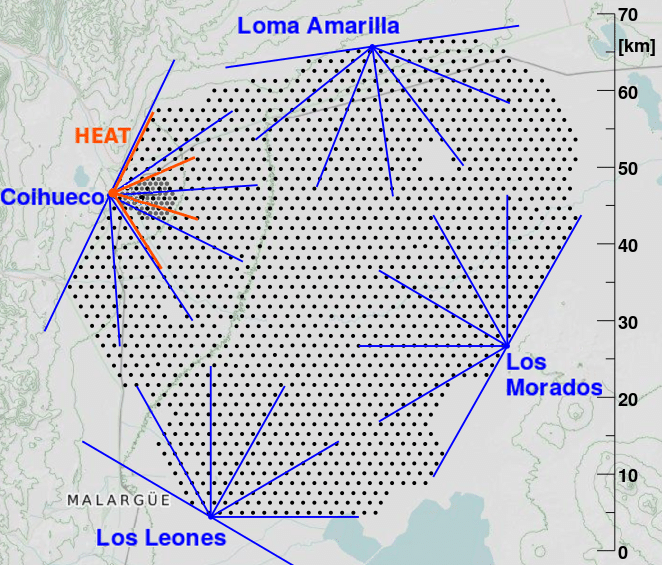
\includegraphics[width=0.4\textwidth]{img/auger_site.png} }}%
    \qquad
    \subfloat[\centering Foto di un detector di Auger.]{{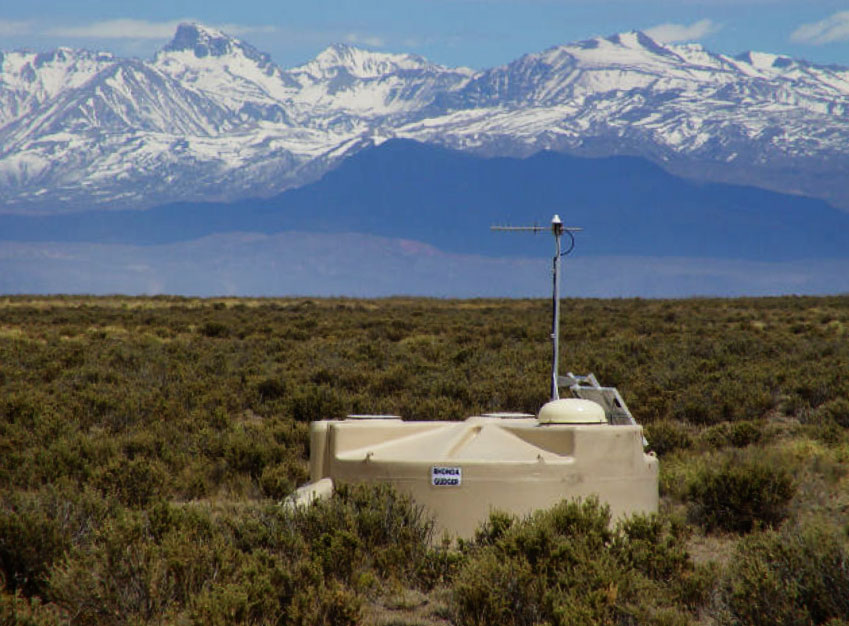
\includegraphics[width=0.45\textwidth]{img/auger_detector.jpg} }}%
    \caption{Immagini dell'esperimento \href{https://www.auger.org}{Auger}, situato in Argentina.}%
    \label{img:auger}
\end{figure}
Ciascun rivelatore contiene acuqa, con un PMT che rivela la luce emessa per effetto Cherenkov. Dalla misura dell'energia depositata nei rivelatori e dal tempo di arrivo del segnale, si riesce a risalire alla direzione di provenienza del raggio cosmico, alla sua energia e, con una certa approssimazione, anche al suo $Z$.

Un altro esempio di esperimento è KASKADE, in Germania. Un array di 252 rivelatori in un'area di $200\times 200\,\textup{m}^2$, ciascun rivelatore consiste in un calorimetro adronico composto di ferro e camere di ionizzazione. Data l'area minore di estenzione dell'esperimento, non è possibile rivelare sciami provenienti da particelle con energia dell'ordine di $10^{20}\,\textup{eV}$.

\begin{figure}[H]
    \centering
    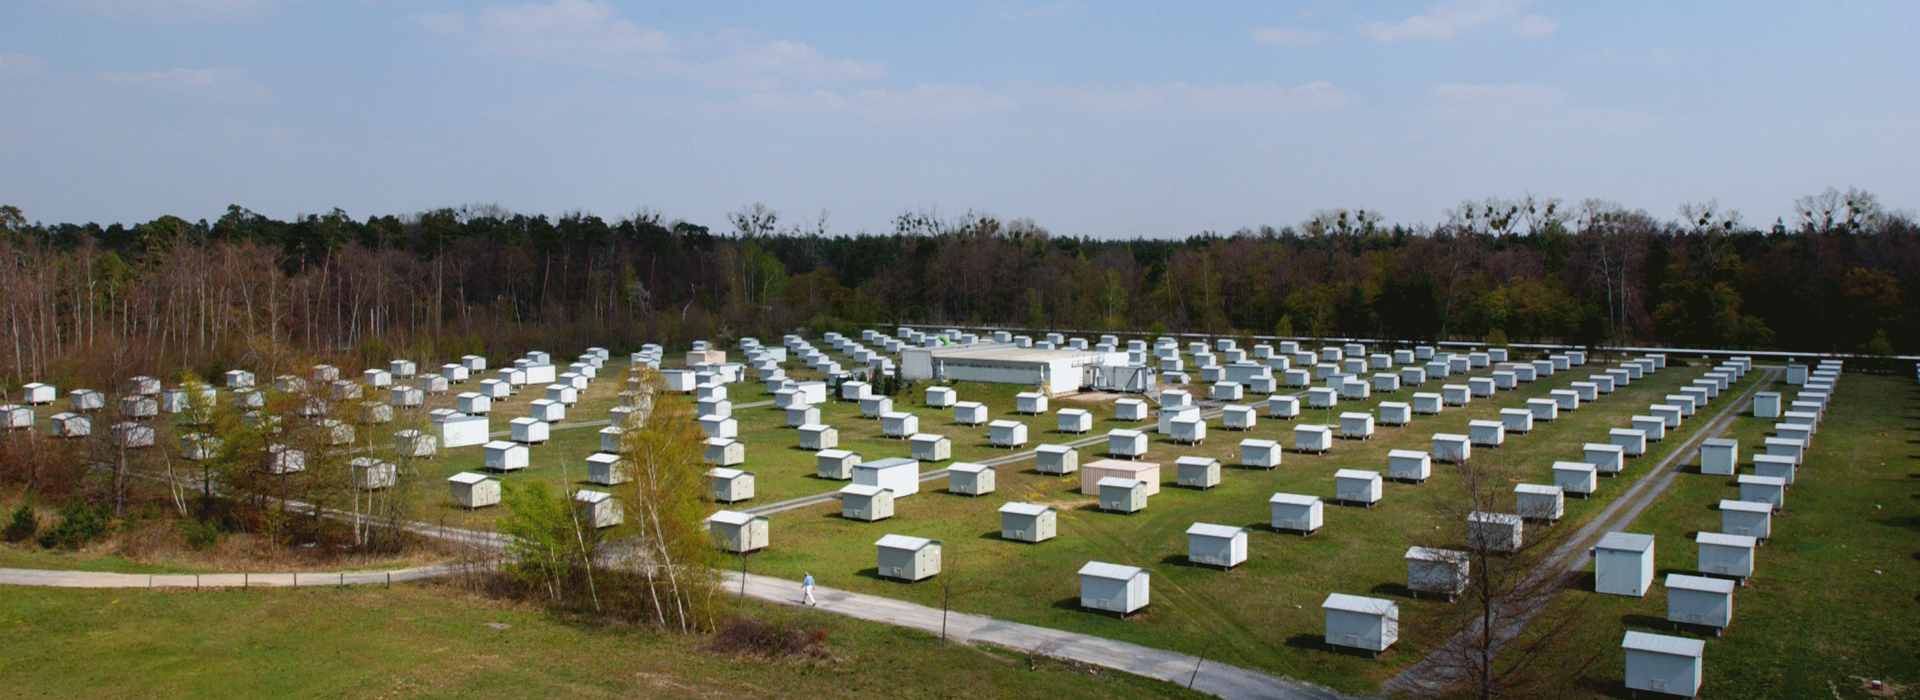
\includegraphics[width=0.6\textwidth]{img/kaskade.jpg}
    \caption{Foto del sito dove si trova KASKADE.}
    \label{img:kaskade}    
\end{figure}

Un altro meccanismo per la rivelazione dei raggi cosmici consiste nel principio di fluorescenza: le particelle cariche presenti negli sciami adronici e elettromagnetici interagiscono con l'azoto dell'atmosfera che transiscono in uno stato eccitato emettendo radiazione nel range $300-400\,\textup{nm}$, quando ritornano nel loro stato fondamentale. Questa radiazione, chiamata \emph{luce di fluorescenza} può attraversare kilometri di atmosfera senza essere assorbita. Per osservarla, come viene fatto nell'esperimento di Auger, si utilizzano dei telescopi: la luce viene raccolta da delle parabole, che la convogliano nel fuoco, dove si trova una matrice di PMT. Per questioni geometrice, ciascun PMT di questa matrice mappa una diversa regione dello spazio. Registrando dunque tempo di arrivo e altezza dell'impulso su ciascun PMT della matrice si riesce a ricostruire l'evoluzione dello sciame e l'energia della particella primaria.

Per completezza, un altro metodo con cui si rivelano i raggi cosmici è attraverso rivelatori di luce Cherenkov, sfruttando il fatto che l'aria si comporta come un mezzo con indice di rifrazione diverso da $1$. Le particelle relativistiche prodotte negli sciami infatti emettono luce Cherenkov, tipicamente una luce blu della durata di pochi $\textup{ns}$.

In alcuni casi è stato possibile effettuare misure di raggi cosmici dallo spazio, montando rivelatori di raggi cosmici su satelliti o stazioni orbitanti. Data la limitata disponibilità di spazio, è possibile osservare solo lo spettro delle basse energie, da confrontare poi con le misure ad alte energie compiute a terra. In questi casi, di esperimenti condotti nello spazio o su palloni, è possibile utilizzare campi magnetici (tipicamente prodotti da superconduttori) per poter discriminare il segno della carica delle particelle che passano dal rivelatore. Dalla misura di curvatura si determinano infatti il segno della carica e l'impulso della particella.

\section{Meccanismi di accelerazione dei raggi cosmici}\index{Accelerazione di raggi cosmici}

Partiamo da un semplice richiamo di un problema fondamentale, ovvero vogliamo studiare la curvatura di una particella carica nello spazio in presenza di un campo magnetico costante e uniforme $\vec{B}$. Partiamo scrivendo
\begin{gather}
    \frac{\der \vec{p}}{\der t} = \frac{Ze}{c}\vec{v} \times \vec{B} = m\frac{\der \gamma}{\der t}\vec{v} + m\gamma \frac{\der \vec{v}}{\der t} = m\gamma \frac{\der \vec{v}}{\der t}, \label{eq:RC1}\\
    \vec{p} = m\gamma \vec{v}. \notag
\end{gather}
Nel piano trasverso deve valere la seguente uguaglianza:
\begin{gather*}
    \biggl| \frac{\der \vec{v}}{\der t} \biggr| = \frac{v_\bot^2}{R},\\
    m\frac{v_\bot^2}{R} = \frac{Ze}{c}v_\bot B,
\end{gather*}
dove abbiamo sostiutito il risultato ottenuto in Eq.(\ref{eq:RC1}). Dunque otteniamo
\begin{equation}
    R = \frac{m\gamma v_\bot c}{ZeB} = \frac{pc}{Ze}\frac{\sin \theta}{B},
    \label{eq:RC2}
\end{equation}
\begin{definition}
    La variabile $R$ ricavata in Eq.(\ref{eq:RC2}) viene chiamata \emph{giroraggio}, mentre il rapporto $\displaystyle\frac{pc}{Ze}$ viene chiamato \emph{rigidità}, questa la si può intendere come la resistenza con cui la particella si oppone all'effetto di curvatura del campo magnetico. 
\end{definition}
\begin{notation}
    In molti testi si riporta con la lettera $R$ sia il giroraggio che la rigidità. Per evitare confusione utilizzeremo la seguente notazione:
    \begin{itemize}
        \item $R$ per il giroraggio,
        \item $\mathcal{R}$ per la rigidità.
    \end{itemize}
\end{notation}

Adesso vogliamo domandarci fino a che energie si possono misurare sui satelliti da una semplice misura di deflezione della traiettoria di una particella in campo magnetico. Il primo taglio, come già detto, è dovuto alla superficie finita disponibile sui satelliti, dunque risulta anche non producente utilizzare campi magnetici intensi a tal punto da curvare sensibilmente particelle che raramente osserveremo. Il secondo limite è imposto dalla risoluzione spaziale con cui riusciamo a misurare la curvatura della traiettoria. Si faccia riferimento alla figura Fig.(\ref{img:giroradius}).

\begin{figure}[H]
    \centering
    %\includegraphics[]{}
    \caption{Schematizzazione del problema.}
    \label{img:giroradius}
\end{figure}

Il campo magnetico presente nel rivelatore è di intensità $| \vec{B}| \sim 1\,\textup{T}$, la risoluzione spaziale è $\delta \sim 10 \,\mu\textup{m}$. La lunghezza del rivelatore lungo la quale la particella passa è di circa $L \sim 1\,\textup{m}$. Possiamo dunque misurare quanto la traiettoria della particella si discosta dalla  traiettoria rettilinea (\emph{sagitta} $s$), nel migliore dei casi misuriamo una distanza $\delta$:
\begin{gather}
    \begin{split}
        s & \sim R - R\cos \frac{\theta}{2} \sim R\frac{\theta^2}{8} \sim R \frac{L^2}{8 R^2}\\
               & \sim \frac{L^2}{8 R},\label{eq:giro1}
    \end{split}\\
    \delta s \sim \frac{L^2}{8}\frac{\delta R}{R^2}.\label{eq:giro2}
\end{gather}
In Eq.(\ref{eq:giro1}) abbiamo utilizzato il fatto che $\theta \ll 1$ e conseguentemente $\theta = L/R$. In Eq.(\ref{eq:giro2}) abbiamo utilizzato l'usuale propagazione degli errori. Da Eq.(\ref{eq:RC2}) notiamo che
\begin{equation*}
    \frac{\delta R}{R} = \frac{\delta p_\bot}{p_\bot},
\end{equation*}
dunque, sostituendo nell'equazione di prima otteniamo
\begin{equation*}
    \delta s = \frac{L^2 ZeB}{8p_\bot c} \frac{\delta p_\bot}{p_\bot},
\end{equation*}
se ad esempio imponiamo che $\delta p_\bot / p_\bot \sim 50\%$ otteniamo che
\begin{equation*}
    (p_\bot c)_\textup{max} = \frac{L^2 ZeB}{8\delta s} 0.5 = 3\,\textup{erg} \simeq 2\,\textup{TeV}. 
\end{equation*}
\begin{example}
    Chiediamoci dunque: un protone con energia di $\sim1\,\textup{TeV}$ quanto è influenzato dal campo magnetico solare? Supponiamo di voler calcolare la sagitta nella curvatura che il protone compie tra il sole e la terra (questo fissa la distanza $L$). Ricordiamo che $L_\textup{sole-terra} = 1\,\textup{UA} \sim 150\times 10^6\,\textup{km}$ e che $|\vec{B}|_\textup{sole} \sim 10\,\mu\textup{G}$. Usando Eq.(\ref{eq:RC2}) per ricavare $R$ e Eq.(\ref{eq:giro1}) per ricavare $s$ si ottiene
    \begin{equation*}
        s = \frac{L^2 ZeB}{8p_\bot c} \simeq 10^{-2}\,\textup{UA}.
    \end{equation*}
\end{example}
Consideriamo adesso la frequenza di rotazione in campo magnetico di una particella, possiamo scrivere la pulsazione come $\omega_\textup{G} = v_\bot / R$, dove $R$ è il giroraggio. Nel caso non relativistico e per carica unitaria possiamo portare avanti il calcolo come segue:
\begin{equation}
    \omega_\textup{G} = \frac{v_\bot}{mv_\bot c}eB = \frac{eB}{mc}. \label{eq:omegagiro}
\end{equation}
Se applichiamo un campo magnetico ad un atomo, questa formula descrive come cambia la frequenza di rotazione attorno al nucleo dell'elettrone. Di fatto corrisponde, se moltiplicato per $\hslash$, all'effetto Zeeman per l'atomo di idrogeno. Nella galassia è presente una grande quantità di idrogeno, osservabile perchè si vede una riga particolare che è quella a $1.4\,\textup{GHz}$ dell'idrogeno neutro. La frequenza di giroraggio risulta dunque essere $\nu_\textup{G} = 29\,\textup{GHz}/\textup{T}$. Dato che il campo magnetico solare è dell'ordine dei $10^{-9}\,\textup{T}$, otteniamo che la frequenza data dall'effetto Zeeman è $29\,\textup{Hz}$. Se modelliziamo l'elettrone classicamente, dunque in orbita intorno al nucleo, abbiamo che a seconda del verso di rotazione (orario o antiorario), il campo magnetico tende a far allontanare o avvicinare l'elettrone, dunque a rallentarlo o ad accelerarlo. Lo splitting di queste due popolazioni è di vitale importanza: conoscere la distanza tra i picchi delle due distribuzioni fornisce informazioni sul campo magnetico presente in quella regione di spazio.

Proviamo adesso a considerare un campo magnetico uniforme (nello spazio) e lentamente variabile, ($\Delta B / B$ piccolo) ovvero una variazione di campo magnetico piccola in un tempo prefissato, che è quello in cui la particella attraversa la regione dove è presente il campo magnetico ($T \simeq 1 / \nu_\textup{G}$). In queste condizioni possiamo considerare la traiettoria della particella come una spira percorsa da corrente, dunque possiamo considerare la corrente $i = Ze / T$. Ricordando Eq.(\ref{eq:omegagiro}), ricavando da questa l'espressione per la frequenza $\nu_\textup{G}$ e sostituendo l'espressione del giroraggio, calcoliamo il momento magnetico di questa spira:
\begin{gather}
    \nu_\textup{G} = \frac{v_\bot}{2\pi R}, \notag \\
    R = \frac{p_\bot c}{ZeB} = \frac{m v_\bot c}{ZeB} \notag \\
    \mu = \frac{iA}{c} = \frac{Ze v_\bot R}{2c} = \frac{1}{2}\frac{mv_\bot^2}{B} = \frac{W_\bot}{B}. \label{eq:mu_spira}
\end{gather}
dove con $W_\bot$ indichiamo l'energia cinetica trasversa. Ci chiediamo quanto vale la variazione del momento magnetico in un giro. Dunque analiziamo la variazione di $\Delta W$ in un giro. Ricordiamo che
\begin{equation*}
    \vec{\nabla} \times \vec{E} = -\frac{1}{c} \frac{\partial \vec{B}}{\partial t},
\end{equation*}
utilizzando le note relazioni tra campi vettoriali otteniamo che 
\begin{equation*}
    \int_{\delta S} \vec{E} \cdot \der \vec{l} = -\frac{1}{c} \int_{S} \frac{\partial \vec{B}}{\partial t},
\end{equation*}
dove con $\delta S$ intendiamo il contorno della superficie su cui integriamo. Il segno negativo davanti al secondo integrale si annulla con considerazioini date dalla regola della mano destra quando andiamo a calcolare il prodotto scalare presente nell'equazione. Utilizziamo l'approssimazione detta prima per il campo magnetico ed otteniamo
\begin{equation*}
    \int_{\delta S} \vec{E} \cdot \der \vec{l} = \frac{1}{c}\frac{\Delta B}{T} \pi R^2.
\end{equation*}
Per ottenere la variazione di energia cinetica scriviamo semplicemente
\begin{gather*}
    \Delta W_\bot = \frac{Ze \Delta B \pi R^2}{cT} = \frac{Ze \Delta B \pi R^2}{c} \frac{v_\bot}{2\pi R} = \frac{Ze\Delta B v_\bot}{2c} \frac{mv_\bot c}{ZeB} = \frac{\Delta B}{B} W_\bot,\\
    \frac{\Delta B}{B} = \frac{\Delta W_\bot}{W_\bot},
\end{gather*}
dove abbiamo sostituito l'espressione di $1/T$ con quella della frequenza di giroraggio, e abbiamo sostituito $R$ con Eq.(\ref{eq:giro2}). Ricordando adesso Eq.(\ref{eq:mu_spira}) otteniamo
\begin{equation*}
    \Delta \mu = \frac{\Delta W_\bot}{B} - W_\bot \frac{\Delta B}{B^2} = \frac{W_\bot}{B}\biggl(\frac{\Delta W_\bot}{W_\bot} - \frac{\Delta B}{B}\biggr) = 0,
\end{equation*}
possiamo dunque dire che $\mu$ in questo caso (campo magnetico lentamente variabile e particella non relativistica) è un invariante adiabatico. Ricaviamo quindi da Eq.(\ref{eq:mu_spira})
\begin{equation}  
    \begin{cases}
        \Delta \biggl(\displaystyle\frac{p_\bot^2}{B}\biggr) = 0, \\
        \Delta (BR^2) = 0,
    \end{cases}
    \label{eq:adiabatico}
\end{equation}
dove l'ultima espressione è stata ottenuta facendo una sostituzione con l'espressione del giroraggio, dalla quale abbiamo ricavato l'espressione per $p_\bot$. In particolare, questa ultima espressione ci dice che l'integrale sull'area del campo magnetico è costante.

\begin{example}[Fasce di Van Allen]
    Il campo magnetico terrestre è un campo magnetico di dipolo, dunque con un addensamento di linee di campo in prossimità dei poli. Se una particella carica a bassa energia arriva in prossimità del campo magnetico terrestre, considerando che localmente possiamo approssimare il campo magnetico terrestre come uniforme, sappiamo che il moto a cui sarà soggetta la particella è di tipo elicoidale. Ricordando la coppia di equazioni Eq.(\ref{eq:adiabatico}), possiamo concludere che in questa prima fase di traiettoria della particella, il raggio dell'elica sarà costante. La particella dunque continua a seguire la linea di campo di $\vec{B}$. Quando la particella procede con la sua traiettoria nella regione più vicina ai poli, dove il campo magnetico si intensifica, se $B$ aumenta, $R$ diminuisce (con $\sqrt{B}$), inoltre sempre da Eq.(\ref{eq:adiabatico}) deve aumentare l'energia cinetica trasversa. Dato che la forza di Lorentz non fa lavoro possiamo scrivere
    \begin{equation*}
        \vec{F} \cdot \vec{v} = 0,
    \end{equation*}
    dunque
    \begin{equation*}
        \sqrt{p_\bot^2 c^2 + p_\parallel ^2 c^2 + m^2 c^4} = \textup{costante}.
    \end{equation*}
    Dovendosi conservare il rapporto $p_\bot^2 / B$ possiamo affermare che la velocità di rotazione attorno alla linea di campo aumenta, diminuisce invece la componente parallela (dovendosi conservare $W$). Scrivendo la relazione 
    \begin{equation*}
        \vec{F} = - \vec{\nabla} (\vec{\mu} \cdot \vec{B})
    \end{equation*}
    si nota subito che se $B$ aumenta, la forza lo respinge e viceversa. Dunque quando la particella si avvicina al polo non solo inizia a girare più velocemente ma ad un certo punto cambia pure direzione. Il comportamento di nostro interesse è infatti quello per cui una particella, quando arriva in una zona con forti campi magnetici, rimbalza. Potremmo dare il nome di \emph{specchi magnetici} a questi tipi di effetti, utilizzati ad esempio per il confinamento di plasmi.
\end{example}

\subsection{Meccanismo di accelerazione di Fermi}
Il primo meccanismo di accelerazione che studiamo è una semplificazione di quello proposto da Enrico Fermi nel 1949. Una particella ultrarelativistica di carica $Ze$ si muove con impulso $\vec{p}$ verso un fronte d'onda di una nube di campo magnetico $\vec{B}$, questa ha una velocità $\vec{v}$, senza perdita di generalità supponiamo $\vec{v}$ diretta lungo la direzione positiva dell'asse $\hat{z}$ e $\vec{p}\cdot\hat{z} < 0$, dunque siamo nello scenario in cui nube magnetica e particella si stanno avvicinando con un certo angolo di inclinazione $\theta$ relativo tra i due. Consideriamo inoltre che la massa della nube sia molto maggiore di quella della particella. Nel sistema di riferimento in quiete con la nube, l'urto tra nube e particella è di tipo elastico, si conserva cioè la componente dell'impulso $\vec{p}_\parallel '$ parallela alla superficie della nube. 

Facendo una trasformazione di Lorentz nel sistema di riferimento in quiete con la nube, possiamo scrivere
\begin{gather*}
    E_i' = \gamma_v (E_i + c\beta_v p_{z, i}),\\
    cp_{z, i}' = \gamma_v (cp_{z, i} + \beta_v E_i),
\end{gather*}
dove con il pedice $v$ si intende il valore di velocità della nube, ricordando che stiamo facendo un boost nel sistema di riferimento della nube, con il pedice $i$ si intende la quantità iniziale. Quello che vogliamo imporre è
\begin{gather*}
    E_f' = E_i',\\
    p_{z, f}' = - p_{z, i}'.
\end{gather*}
Siamo interessati all'energia finale della particella nel sistema di riferimento del laboratorio:
\begin{equation*}
    \begin{split}
        E_{f} & = \gamma_v (E_{f}' - c\beta_v p_{z,i}') = \gamma_v (E_i' + c\beta_v p_{z,i}')\\
              & = \gamma_v (\gamma_v (E_i + c\beta_v p_{z,i}) + \beta_v \gamma_v (cp_{z, i} + \beta_v E_i))\\
              & = \gamma_v^2 E_i + 2 \gamma_v^2 \beta_v c p_{z, i} + \gamma_v^2 \beta_v^2 E_i \\
              & = \gamma_v^2 (E_i + 2 \beta_v c p_{z, i} + \beta_v^2 E_i) \\
              & \simeq (1+\beta_v^2 ) (\cdots),
    \end{split}
\end{equation*}
esplicitando i calcoli per $E_f - E_i$, lasciando solo i termini al primo ordine in $\beta_v^2$, otteniamo che
\begin{equation}
    \frac{\Delta E}{E} = 2 \beta_v^2 + 2 \beta_v \frac{p_ic}{E}\cos \theta \simeq 2 (\beta_v^2 + \beta_v \cos \theta). \label{eq:betavcoshtheta}
\end{equation}
dove abbiamo utilizzato il fatto che $p_i c / E = \beta \simeq 1$. Aggiungiamo adesso la complicazione che i fronti d'onda che la particella incontrerà saranno in numero maggiore di 1, consideriamo per il momento che il passo tra un fronte e il successivo sia $\lambda$. Se le velocità della particella e delle nubi sono $\vec{v}$ e $\vec{V}$ con un angolo relativo $\theta$, possiamo scrivere che la velocità realtiva è
\begin{equation*}
    v_\textup{rel} = \frac{v\cos \theta + V}{1 + \frac{vV}{c^2}\cos \theta},
\end{equation*}
se le due velocità sono concordi invece
\begin{equation*}
    v_\textup{rel} = \frac{v\cos \theta - V}{1 - \frac{vV}{c^2}\cos \theta}.
\end{equation*}
Se approssimiamo la prima delle due in $V/c$, proprio come prima abbiamo fatto con $\beta_v$, otteniamo
\begin{equation}
    \begin{split}
        v_\textup{rel} & \simeq (v\cos \theta + V)\biggl(1 - \frac{vV}{c^2} \cos \theta \biggr) = v \cos \theta + V \sin^2 \theta \label{eq:thetaaverage} \\
                       & \simeq 
                        \begin{cases}
                            c (\cos \theta + \frac{V}{c} \sin^2 \theta), \quad \cos \theta > 0 \\
                            - c (\cos \theta - \frac{V}{c} \sin^2 \theta), \quad \cos \theta < 0
                        \end{cases}
    \end{split}
\end{equation}
Adesso dunque vogliamo mediare Eq.(\ref{eq:betavcoshtheta}) sulla funzione di $\cos\theta$ di Eq.(\ref{eq:thetaaverage}). Faccio dunque il valore di aspettazione, normalizzando per la funzione distribuzione di $\theta$
\begin{equation*}
    \mathbb{E}\biggl[\frac{\Delta E}{E}\biggr] = \frac{\int_{-1}^{+1}\frac{\Delta E}{E} v_\textup{rel}(\cos \theta) \der \cos \theta}{\int_{-1}^{+1}v_\textup{rel}(\cos \theta) \der \cos \theta} = \frac{V}{c} = \beta_v.
\end{equation*}
Abbiamo ottenuto il risultato integrando correttamente sulle diverse regioni di $v_\textup{rel}$, usando inoltre la parità/disparità dei vari termini si velocizzano i calcoli. Dunque abbiamo ottenuto che $\Delta E / E \simeq 3 \beta_v^2 \equiv \xi $, dopo un rimbalzo la particella ha energia $E_1 = E_0 (1 + \xi)$, dopo $n$ rimbalzi ha energia $E_n = E_0 (1 + \xi)^n$. Siamo adesso interessati a calcolare la probabilità che una particella con una certa energia iniziale $E_0$ raggiunga una energia fissata $\overline{E}$. Iniziamo osservando che 
\begin{equation}
    \overline{n} = \frac{\ln \overline{E} / E}{\ln (1+ \xi)},\label{eq:overline_n}
\end{equation}
dunque dobbiamo chiederci quanto valga la probabilità che la particella riesca a fare più di $\overline{n}$ rimbalzi. Data la probabilità di fuga $p_\textup{F}$, la probabilità di rimanere intrappolata nel meccanismo di accelerazione per $n$ volte varrà $(1 - p_\textup{F})^n$. Ricollegandoci alla domanda precedente, siamo ora interessati a calcolare la probabilità 
\begin{equation*}
    \Pr (E > \overline{E}) = \sum_{i = \overline{n}} ^{\infty} (1 - p_\textup{F})^i = \frac{(1 - p_\textup{F})^{\overline{n}}}{p_\textup{F}},
\end{equation*}
dove abbiamo utilizzato la proprietà della serie geometrica per ricavare il risultato finale. Se moltiplichiamo questa quantità per il numero inziale di particelle otteniamo una stima di quante particelle hanno almeno energia $\overline{E}$
\begin{equation*}
    \textup{N} (E > \overline{E}) = \alpha \frac{(1 - p_\textup{F})^{\overline{n}}}{p_\textup{F}},
\end{equation*}
se adesso sostituiamo l'espressione di $\overline{n}$ di Eq.(\ref{eq:overline_n}) e ricaviamo nuovamente $\textup{N}$, otteniamo
\begin{equation*}
    \textup{N} (E > \overline{E}) = D \biggl(\frac{\overline{E}}{E}\biggr)^{\ln(1 - p_\textup{F}) / \ln (1 + \xi)} \equiv D \biggl(\frac{\overline{E}}{E}\biggr) ^ {-\gamma},
\end{equation*}
Dove $D$ tiene di conto di tutte le costanti moltiplicative e $\gamma$ è un fattore all'esponente. Derivando questra equazione otteniamo la forma 
\begin{equation}
    \frac{\der N}{\der E} \varpropto E^{- (\gamma + 1)}.\label{eq:gammaplusone}
\end{equation}
Riguardo $\gamma$ possiamo dire
\begin{equation*}
    \gamma = \frac{\ln(1 - p_\textup{F})}{\ln ( 1 + \xi)} \simeq \frac{p_\textup{F}}{\xi},
\end{equation*}
dovremmo quindi confrontare l'espressione dell'esponente in Eq.(\ref{eq:gammaplusone}) con il valore sperimentale osservato ($\simeq 2.7$), riguardante Fig.(\ref{img:cosmicrays}), dunque imporremo $\gamma \simeq 1.7$. Si ricava quindi un valore approssimato per la probabilità di fuga $p_\textup{F} \simeq \gamma / \xi \simeq 1.7 \cdot 3 \times 10^{-8} = 5.1 \times 10^{-8}$. Qundi per arrivare ad energia $\overline{E}$ deve fare, con i valori di $\xi = 3 \times 10^{-8}$ e $\overline{E} = 1\,\textup{TeV}$, $\overline{n} \simeq 4 \times 10^{8}$ rimbalzi. Per capire se questo processo è possibile o meno, ricordiamo che nelle ipotesi iniziali del problema abbiamo detto che i fronti d'onda distano $\lambda$ l'uno dal successivo e che la velocità della nostra particella è $\sim c$, dunque possiamo dare una stima della distanza percorsa dalla particella prima di raggiungere l'energia $\overline{E}$. Prima di fare ciò occorre capire quanto vale $\lambda$: le sorgenti di questi tipi di fenomeni sono tipicamente i residui di supernova, che hanno dimensioni tipiche del \emph{parsec} (circa $3$ anni-luce). Dunque per far avvenire un processo di accelerazione possiamo calcolare $t_\textup{acc} = \lambda / c \simeq 3\,\textup{years}$, il tempo necessario totale sarà $t_\textup{tot} = t_\textup{acc} \cdot \overline{n} = 1.2\times10^{9}\,\textup{years}$.
Una delle caratteristiche misurabili dei raggi cosmici è la composizione isotopica, ad esempio del $^{10}\textup{Be}$, con una vita media di $10^6\,\textup{years}$. Se ne misura la composizione isotopica in relazione con gli altri isotopi, e osserviamo che, essendo in grado di conoscerne la percentuale nel punto di produzione, posso misurare la composizione in un secondo momento per stimare il tempo trascorso. Dalle nostre misure sulla percentuale di $^{10}\textup{Be}$ si stima che il tempo di percorrenza sia $10^7\,\textup{years}$, quindi la stima ricavata prima di $t_\textup{tot}$ risulta errata poichè incompatibile con la vita media dell'isotopo stesso.
Il fattore che fa aumentare $\overline{n}$ nel nostro caso è la dipendenza al denominatore di $\beta_v^2$.

\section{Meccanismo di accelerazione di shock}
Il meccanismo di accelerazione di Fermi presenta due inconvenienti: c'è una dipendenza al numeratore da $\beta_v^2$ e non è nota a priori la probabilità di fuga $p_\textup{F}$. In questo nuovo caso consideriamo un'onda d'urto di shock, lo facciamo nel caso monodimensionale, fronte d'onda piano infinito, che si propaga in un mezzo (ad esempio gas di protoni) con una velocità $\vec{u}$ molto superiore alla velocità del suono nel mezzo $c_\textup{s}$. Il fronte d'urto supponiamo si muova verso destra, dividiamo lo spazio in due zone: la prima a valle del fronte d'urto, la seconda a monte del fronte d'urto. Ci mettiamo nel sistema di riferimento solidale con il fronte d'onda, quindi la porzione di spazio a valle del fronte d'onda si avvicina con velocità $v_1 = u$, il gas a monte ha velocità $v_2$. Le due parti di spazio hanno inoltre rispettivamente le grandezze $\rho_1$, $T_1$ e $p_1$, $\rho_2$, $T_2$ e $p_2$. Nell'attraversamento del fronte d'onda di shock vogliamo imporre la conservazione delle grandezze di massa, impulso ed energia del fluido di protoni.

Data l'assenza di alcuna fonte di materia, impulso o di energia abbiamo
\begin{gather}
    \rho_1 v_1 = \rho_2 v_2,\notag \\
    p_1 + \rho_1 v_1^2 = p_2 + \rho_2 v_2^2, \label{eq:cont2shock}\\
    \rho_1 v_1 \biggl( \frac{1}{2}v_1^2 + h_1 \biggr) = \rho_2 v_2 \biggl( \frac{1}{2}v_2^2 + h_2 \biggr).\label{eq:cont3shock}
\end{gather}
Dagli approfondimenti trattati in App.(\ref{chap:app1}), possiamo semplificare questo sistema scrivendo che
\begin{equation*}
    \begin{cases}
        \displaystyle h = \epsilon + pV = \mu c_\textup{v} T + pV= \frac{c_\textup{v}}{c_\textup{p} + \textup{v}} pV + pV = pV \frac{\gamma}{\gamma - 1}\\
        pV = \mu R T 
    \end{cases},
\end{equation*}
inoltre posso scrivere che 
\begin{equation*}
    v = \frac{\textup{cost}}{\rho} \equiv J V,
\end{equation*}
dopo alcune sostituzioni otteniamo che Eq.(\ref{eq:cont2shock}) ci permette di ricavare il valore di $J$
\begin{equation*}
    J^2 = \frac{p_1 - p_2}{V_2 - V_1}.
\end{equation*}
Eq.(\ref{eq:cont3shock}) ci permette invece di scrivere
\begin{equation*}
    h_1 - h_2 = -\frac{1}{2}J^2(V_1^2 - V_2^2),
\end{equation*}
possiamo sostituire ad $h$ e $J^2$ le espressioni ricavate prima ed ottenere
\begin{equation*}
    \frac{\gamma}{\gamma - 1} (p_1 V_1 - p_2 V_2) + \frac{1}{2}(p_1 - p_2)(V_1 + V_2) = 0.
\end{equation*}
Possiamo dunque ricavarici il seguente rapporto
\begin{equation}
    \frac{V_2}{V_1} = \frac{(\gamma + 1)p_1 + (\gamma - 1)p_2}{(\gamma + 1)p_2 + (\gamma - 1)p_1},\label{eq:V2fracV1}
\end{equation}
sostituendo nell'espressione di $J^2$ questo rapporto otteniamo
\begin{equation*}
    J^2 = \frac{(\gamma + 1)p_2 + (\gamma - 1)p_1}{2V_1}.
\end{equation*}
Possiamo adesso scrivere l'espressione di $v_1^2$
\begin{equation}
    v_1^2 = J^2 V_1^2 = \frac{V_1}{2}\bigl[ (\gamma + 1)p_2 + (\gamma - 1)p_1 \bigr].\label{eq:v_1^2}
\end{equation}
\begin{definition}[Numero di Mach]
    Il rapporto tra la velocità $v$ di un oggetto nel fluido e la velocità del suono $c_\textup{s}$ nel fluido è chiamato \emph{numero di Mach}
    \begin{equation*}
        M \equiv \frac{v}{c_\textup{s}}
    \end{equation*}    
\end{definition}
In App.(\ref{chap:app1}) abbiamo trovato che 
\begin{equation*}
    c_{\textup{s}, i} = \sqrt{\gamma \frac{p_i}{\rho_i}}
\end{equation*}
per il fluido $i$-esimo. Nel nostro caso abbiamo
\begin{equation*}
    M_1^2 = \frac{v_1^2}{\gamma p_1 V_1},
\end{equation*}
in Eq.(\ref{eq:v_1^2}) abbiamo ricavato l'espressione per $v_1^2$, possiamo sostituire ed ottenere
\begin{equation*}
    M_1^2 = \frac{(\gamma + 1)p_2 + (\gamma - 1)p_1}{2 \gamma p_1},
\end{equation*}
si nota dunque che possiamo scrivere il numero di Mach come funzione unicamente del rapporto tra le pressioni a valle e a monte del fronte d'onda di shock
\begin{equation*}
    \frac{p_2}{p_1} = \frac{2 \gamma M_1^2 - (\gamma - 1)}{\gamma + 1}.
\end{equation*}
Si nota ad esempio che se $M$ tende a $+\infty$, si ha che la pressione nella zona a monte è molto maggiore di quella a valle.

Vogliamo invece trattare adesso il caso analogo ma per le desità e le velocità. Consideriamo ad esempio 
\begin{equation*}
    \frac{\rho_2}{\rho_1} = \frac{V_1}{V_2} = \frac{v_1}{v_2} = \frac{1 + \gamma}{(\gamma - 1) + \frac{2}{M_1^2}},
\end{equation*}
dove al terzo passaggio abbiamo sfruttato la conscenza del rapporto $p_2 / p_1$ e la relazione di Eq.(\ref{eq:V2fracV1}). In questo caso, se $M_1^2$ tende a $+\infty$ abbiamo che $V_1/V_2$ tende a un rapporto finito $(\gamma + 1) / (\gamma - 1)$, che per il gas di protoni (monoatomico) vale $4$. Abbiamo quindi trovato che in caso ultrasonico, la velocità nella zona a monte vale $v_2 = u/4$ . È possibile verificare sperimentalmente questi dati osservando i residui di supernovae. Inoltre, nello stesso limite per $M_1^2$ possiamo scrivere
\begin{equation*}
    \frac{T_2}{T_1} = \frac{p_2V_2}{p_1V_1} \varpropto M_1^2
\end{equation*}

Consideriamo il sistema di riferimento solidale con il gas di protoni a valle del fronte d'urto. Il fronte d'urto si muove verso destra con velocità $\vec{u}$. Il gas che si trova a monte si muove verso destra con velocità $\frac{3}{4}\vec{u}$, per convincersi basti pensare che la velocità relativa è $\frac{3}{4}u$. Poniamoci nel punto di vista della particella a valle che passando il fronte d'urto si ritrova nella zona a monte. Supponiamo che l'interazione avvenga con il campo magnetico. La particella che segue questa successione di eventi si ritrova nella parte a monte, dove la velocità del fluido è $\frac{3}{4}\vec{u}$. Dal punto di vista della parte a monte, la parte a valle si dirige verso la parte a monte con velocità $-\frac{3}{4}\vec{u}$, vedendosi arrivare addosso una nube elettromagnetica. In generale può avvenire lo stesso meccanismo di attraversamento del fronte d'urto. Dunque, che la particella si trovi a monte o a valle, si vede in ogni caso avvicinare la frazione di spazio complementare con velocità $\mp\frac{3}{4}\vec{u}$. L'attraversamento del fronte d'urto può in effetti avvenire più di una volta e quello che vogliamo fare adesso è calcolare il guadagno di energia per ogni attraversamento. L'unica accortezza da tenere è che nel caso del sistema di riferimento solidale con la parte a monte, la velocità del fronte d'urto vale $\frac{1}{4}\vec{u}$.

Poniamo dunque che la particella si trovi nella parte a valle. L'energia della particella nel sistema di riferimento della nube che si trova a monte vale
\begin{equation*}
    E' = \gamma_v(E + \beta_v pc \cos \theta),
\end{equation*}
dove $\theta$ è l'angolo relativo tra $\vec{p}$ (impulso della particella) e $\vec{u}$. Rinunciamo all'ipotesi di rimbalzo elastico: la particella viene infatti isotropizzata nella parte a monte e l'angolo di emissione sarà in generale diverso da $\theta$. Approssimando al primo ordine in $\beta_v$ possiamo scrivere $\gamma_v \sim 1$. Ricaviamo immediatamente che 
\begin{equation*}
    \frac{\Delta E}{E} \simeq \beta_v \frac{pc}{E} \cos \theta \simeq \beta_v \cos \theta.
\end{equation*}
Vogliamo dunque ricavare la probabilità che la particella, vada ad urtare contro la superficie. Per fare ciò notiamo che il risultato è semplicemente dato dal numero di particelle che sono contenute nel cilindro che interseca la superficie del fronte d'urto
\begin{equation*}
    N = n c \cos \theta s \Delta t,
\end{equation*}
dove $n$ è la densità del fluido, $c$ la velocità della particella dato che siamo in approssimazione ultrarelativistica e $s$ è la superficie che interseca il cilindro che ho considerato. Per ottenere la probabilità basterà mediare la funzione di prima con questa distribuzione, opportunamente normalizzata
\begin{equation*}
    \displaystyle\Pr(\textup{attraversamento}) \varpropto \frac{\displaystyle\int_0^{\frac{\pi}{2}}\cos^2 \theta \der \cos \theta}{\displaystyle\int_0^{\frac{\pi}{2}}\cos \theta \der \cos \theta} = \frac{2}{3}.
\end{equation*}
Si noti che la differenza sostanziale con il meccanismo di Fermi è che in questo caso non abbiamo supposto una successione di fronti d'urto a distanza $\lambda$, in questo nuovo meccanismo (capito intorno agli anni '70) le particelle attraversano più volte lo stesso fronte d'urto. Se la particella attraversa doppiamente il fronte d'urto (dunque dalla parte a valle si ritrova nuovamente nella parte a valle) abbiamo che
\begin{equation*}
    \frac{\Delta E}{E} = 2 \frac{2}{3} \beta_v = \frac{4}{3}\beta_v = \frac{4}{3}\frac{3}{4}\frac{u}{c} \equiv \xi,
\end{equation*}
infatti il calcolo che andrebbe fatto per l'attraversamento da zona a monte a zona a valle è in questo caso perfettamente simmetrico al calcolo fatto per l'attraversamento da valle a monte, questo spiega il fattore $2$ nell'ultima espressione. Con questo meccanismo è inoltre possibile calcolarsi la probabilità di fuga $p_\textup{F}$. Per impostare il calcolo si noti che 
\begin{itemize}
    \item mentre la particella si trova a valle, questa si vede arrivare il fronte d'urto a velocità $\vec{u}$, attraverserà sicuramente il fronte,
    \item mentre la particella si trova a monte, il fronte si allontana con velocità $\frac{1}{4}\vec{u}$. 
\end{itemize}
Bisogna considerare il flusso delle particelle del secondo caso
\begin{equation*}
    n \int_0^{\frac{\pi}{2}} \frac{c\cos \theta der \Omega}{4\pi} = \frac{nc}{4} \equiv J_\textup{p},
\end{equation*}
questo è il flusso $J$ che urtano sulla superficie. Il flusso di particelle che fuggono sarà invece $\frac{nu}{4}$, dunque la probabilità di continuare a sbattere contro il fronte d'urto vale 
\begin{equation*}
    \Pr = \frac{nc / 4}{(nc/4) + (nu/4)} = \simeq 1 - \frac{u}{c},
\end{equation*}
dunque la probabilità di fuga è $u/c$, svolgendo calcoli simili a quelli del meccanismo di Fermi otteniamo che
\begin{equation*}
    \frac{\der N}{\der E} \varpropto E^{-2}.
\end{equation*}

\section{I luoghi di accelerazione nell'universo}
In Fig.(\ref{img:snr}) si osservano alcune foto di residui di supernovae dove si pensa che abbia luogo il meccanismo di accelerazione di raggi cosmici.
\begin{figure}[H]
    \centering
    \subfloat[\centering SN 1542]{{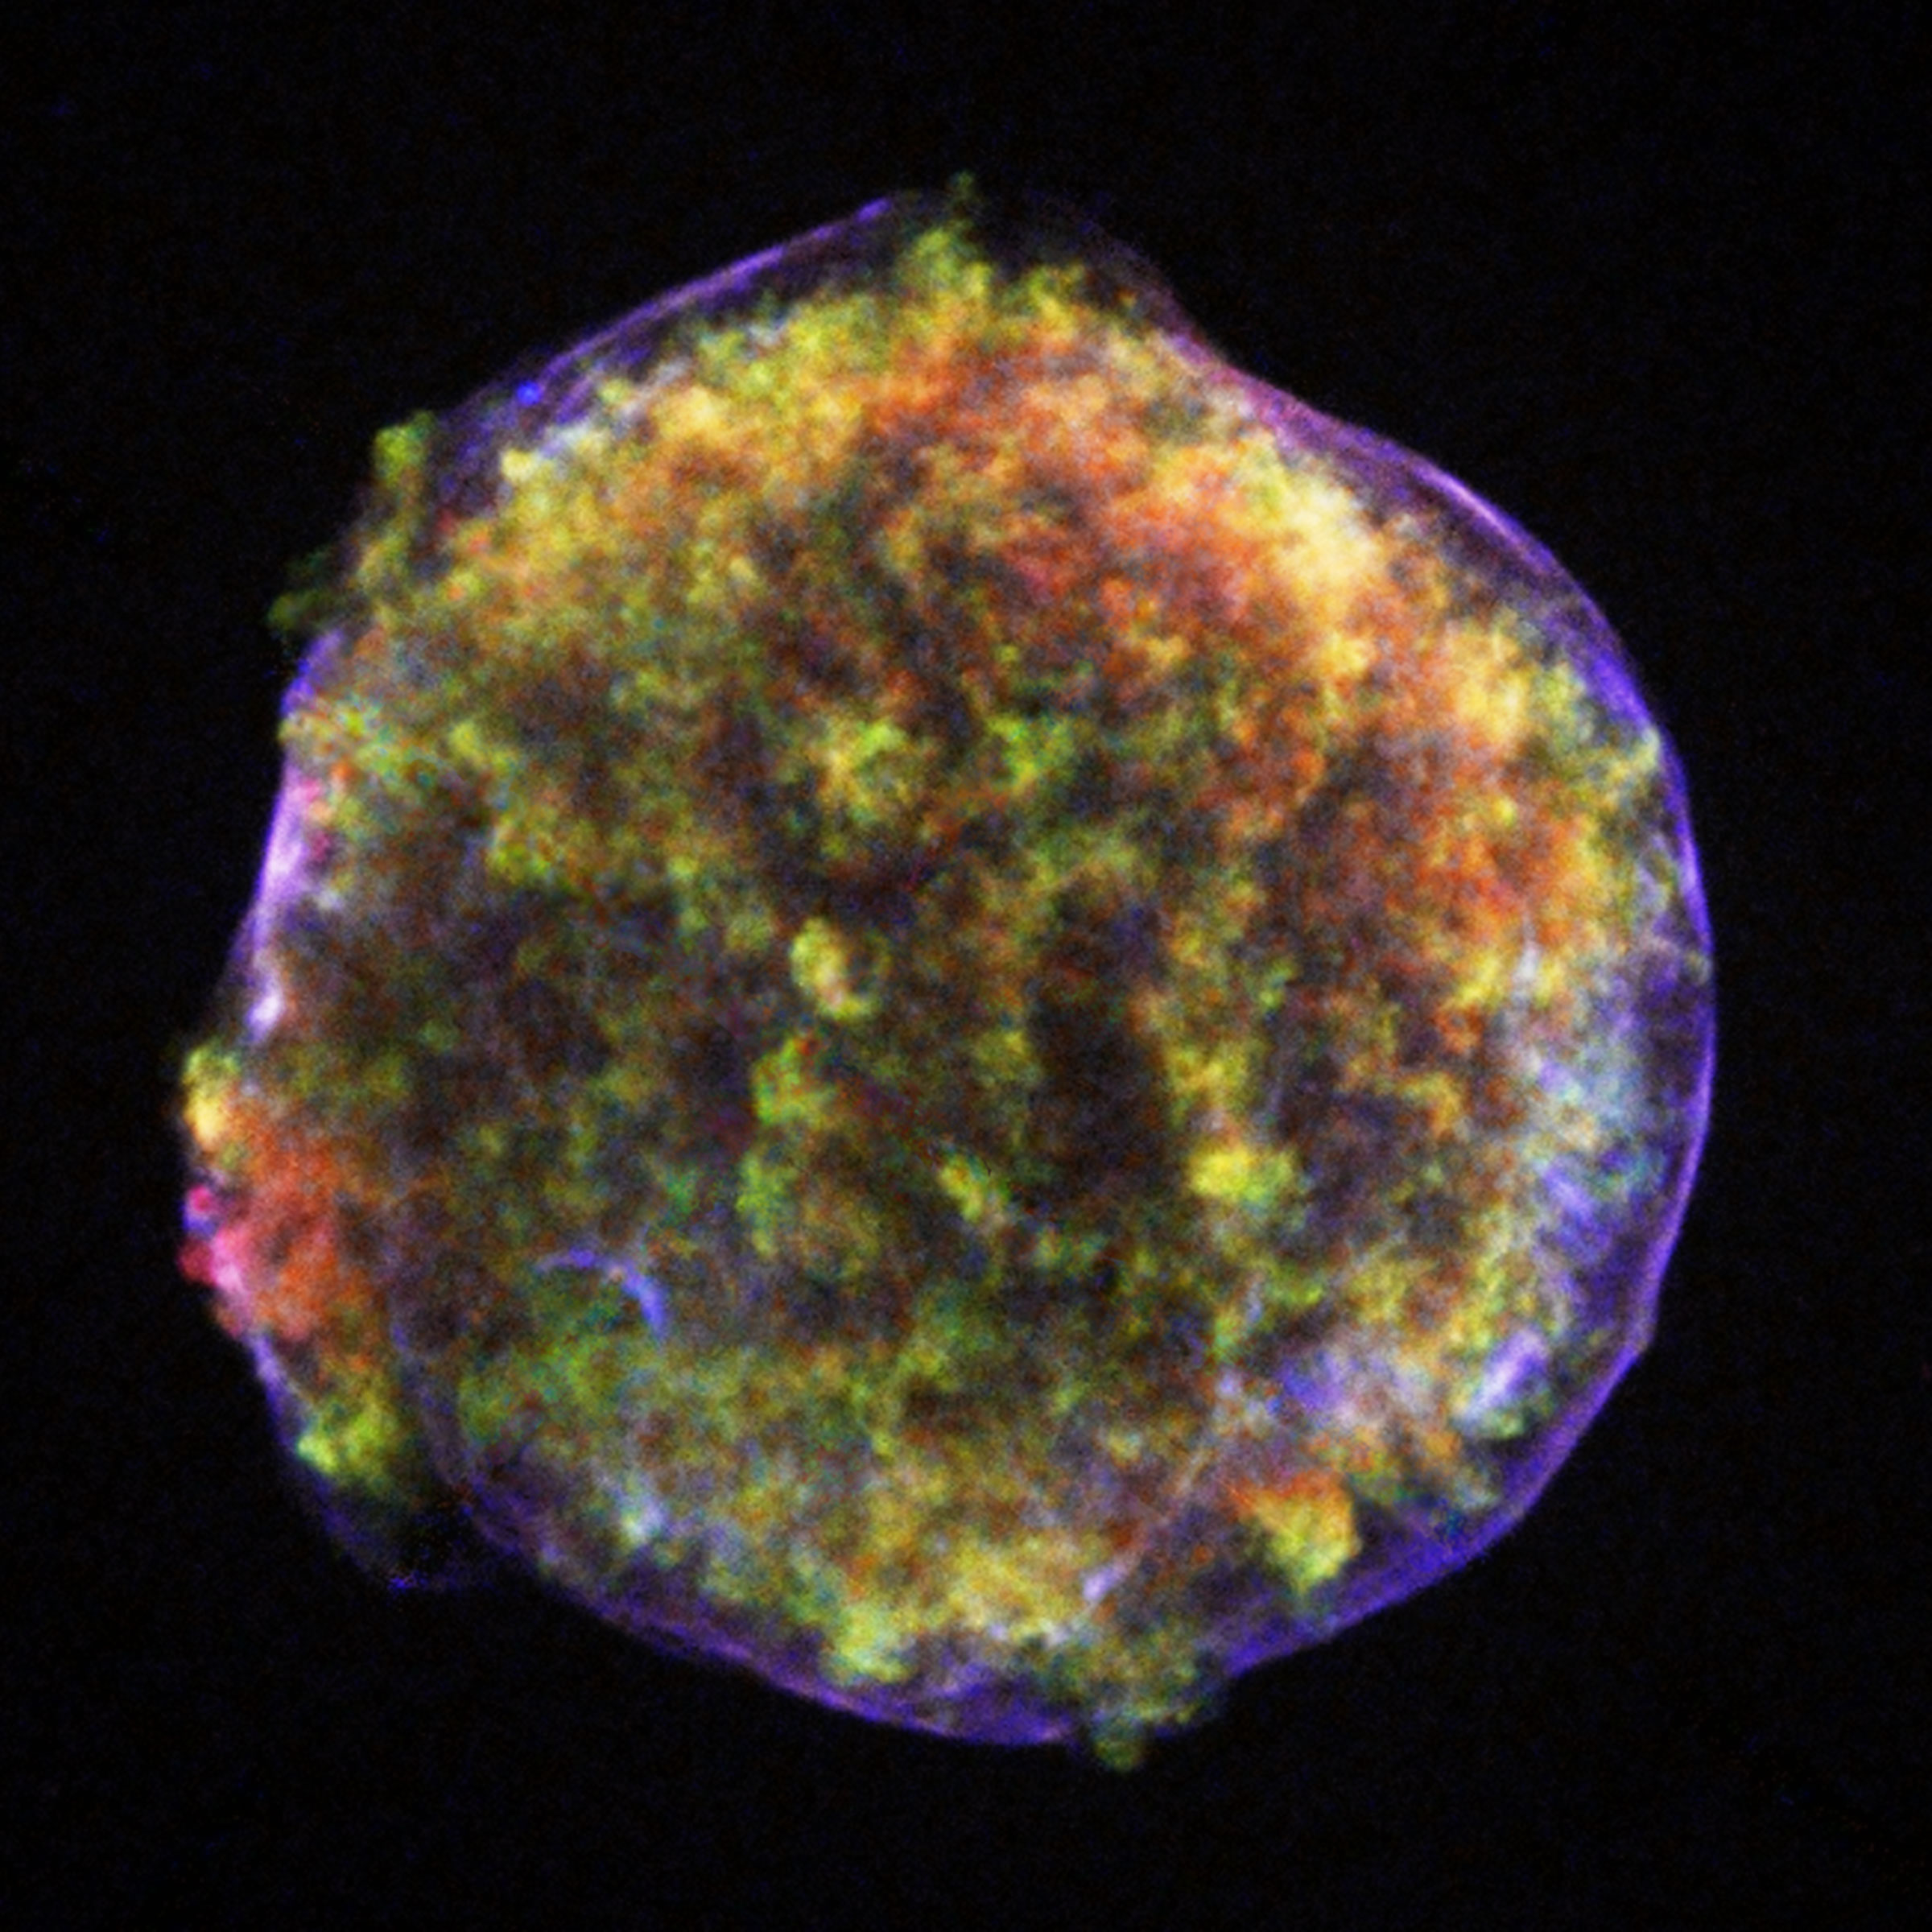
\includegraphics[width=0.3\textwidth]{img/Tycho-supernova-xray.jpg}}}%
    \quad
    \subfloat[\centering Nebulosa del Granchio]{{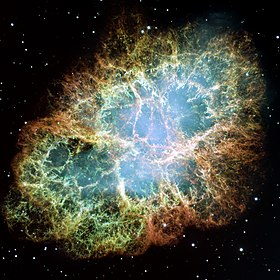
\includegraphics[width=0.3\textwidth]{img/Crab_Nebula.jpg}}}%
    \caption{A sinistra immagine ai raggi X della supernova Tycho, a distanza di $10\,\textup{k a.l.}$, di tipo Ia. A destra immagine nello spettro visibile della Nebulosa del Granchio (1052), a distanza di $6\,\textup{k a.l.}$, di tipo II.}%
    \label{img:snr}    
\end{figure}
Questi, come altri esempi (vedi la nebulosa Keplero 1604), sono appunto solo ipotizzati essere i centri di accelerazione dei raggi cosmici. L'unico modo per avere una certezza consiste nell'osservare raggi cosmici provenienti direttamente da questi siti, ma data la presenza di un campo magnetico non nullo nella galassia questi sarebbero sicuramente deviati. L'obiettivo dunque è quello di osservare particelle neutre provenienti da questi siti, in quanto non soggette a forza di Lorentz. Dato che, come abbiamo accennato, in questi luoghi c'è un'alta concentrazione di protoni, la speranza è di avere in seguito ad un urto la produzione di $\pi^0$ che, decadendo elettromagneticamente, dà origine a due fotoni. L'osservazione di questi fotoni può dunque darci informazione sui meccanismi di accelerazione e sui siti dove questi meccanismi hanno luogo. L'esperimento di FermiLAT ha misurato lo spettro in energia dei fotoni provenienti dai residui di supernova.
\subsection{Altri meccanismi di accelerazione}
Oltre ai residui di supernova, si ipotizza che ci siano altri meccanismi di accelerazione dei raggi cosmici:
\begin{itemize}
    \item pulsar, scoperte nel 1967,
    \item stelle di neutroni, che hanno campi magnetici intensi.
\end{itemize}

\subsubsection*{Argomento di Syrovatskii}
Se consideriamo una pulsar in rapida rotazione, questa può essere modellizzata come una spira di lato $L$, con un campo magnetico rotante di intensità $B$. Come sappiamo dalle equazioni di Maxwell, una variazione di campo magnetico dà origine ad un campo elettrico. Schematizzando il problema come in Fig.(\ref{img:syro}), possiamo scrivere la seguente equazione
\begin{equation*}
    \vec{\nabla} \wedge \vec{E} = - \frac{1}{c}\frac{\partial \vec{B}}{\partial t},
\end{equation*}
data la schematizzazione del problema possiamo semplificare come seguente
\begin{equation*}
    4 \overline{E} L = \frac{1}{c} \frac{\Delta B}{\Delta t} L^2 = \frac{\omega}{c} B L^2.
\end{equation*}
Possiamo dunque ricavare il massimo valore del lavoro che può essere compiuto su una particella di carica $e$
\begin{equation*}
    \epsilon_\textup{MAX} = e \overline{E} L = \frac{eBL}{4} = \textup{O}(10^{20}\,\textup{eV}).
\end{equation*}

\begin{figure}[H]
    \centering
    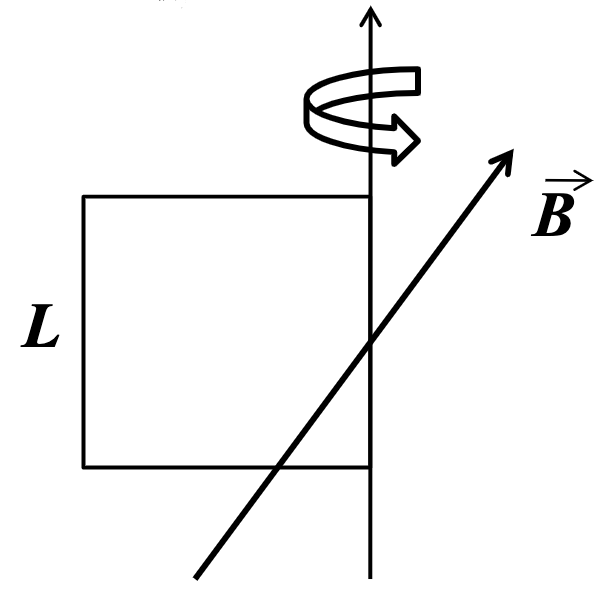
\includegraphics[width=0.4\textwidth]{img/syro.png}
    \caption{Schematizzazione del problema.}
    \label{img:syro}    
\end{figure}

\section{Taglio GZK}

Abbiamo visto che ad alte energie lo spettro in energia dei raggi cosmici ha una incurvatura. Per spiegare questo fenomeno è stato ipotizzato che le particelle cariche ad alta energia interagiscano con la radiazione cosmica di fondo con un processo di produzione di soglia di questo tipo
\begin{equation*}
    p + \gamma \rightarrow \Delta^+ \rightarrow N + \pi.
\end{equation*}
La particella $\Delta^+$ è una risonanza, nel senso che la sua sezione d'urto ha la forma lorentziana. Con un semplice calcolo di cinematica si ricava che l'energia di soglia del protone per far avvenire la produzione della $\Delta^+$ vale circa $10^{21}\,\textup{eV}$. Succede dunque che ad ogni produzione di particella $\Delta^+$, una frazione di energia pari a circa $1/10$ venga persa dal protone nella produzione di pioni. Considerando il numero massimo di urti che possono avvenire con questa cinematica (al massimo una decina), possiamo ricavare da prima il cammino libero medio dei protoni e dunque la distanza massima che questi possono percorrere nell'universo. Il cammino libero medio in questo caso vale
\begin{equation*}
    \lambda = \frac{1}{n\sigma} \sim 10 \,\textup{Mpc},
\end{equation*}
dove per $n$ abbiamo usato la densità di uno spettro di corpo nero, per $\sigma$ usiamo il valore sperimentale di $10^{-28} \,\textup{cm}^2$. Si ricava dunque che la distanza massima percorribile da queste particelle vale circa $100\,\textup{Mpc}$. Questa distanza implica un \emph{taglio} oltre il quale l'universo diventa opaco, questo taglio viene chiamato \emph{taglio GZK}.
\chapterimage{img/SuperKK.jpg} % Chapter heading image
\chapterspaceabove{6.75cm} % Whitespace from the top of the page to the chapter title on chapter pages
\chapterspacebelow{7.25cm} % Amount of vertical whitespace from the top margin to the start of the text on chapter pages

%------------------------------------------------

\chapter{Neutrini}

\section{Produzione nel sole di neutrini}
Il principale meccanismo di produzione di neutrini all'interno di una stella, come il sole, è il meccanismo di fusione. Ad esempio i seguenti processi danno luogo alla produzione di neutrini
\begin{gather*}
    p + p \rightarrow d + e^+ + \nu_e \\
    4p \rightarrow ^4\textup{He} + 2e^+ + 2\nu_e.
\end{gather*}
In particolare si noti che la massa del nucleo prodotto ha una massa più piccola della massa totale dei reagenti, la massa in eccesso rende possibile la produzione di neutrini. A proposito di questo, si potrebbe studiare l'andamento del difetto di massa per nucleone costruendo la seguente funzione
\begin{equation*}
    f = \frac{(m_n(A-Z) + m_p Z - m_N)c^2}{A},
\end{equation*}
questa funzione è calcolabile per ogni nucleo $(A, Z)$, in particolare si veda Fig.(\ref{fig:nuclei}).
\begin{figure}[H]
    \centering
    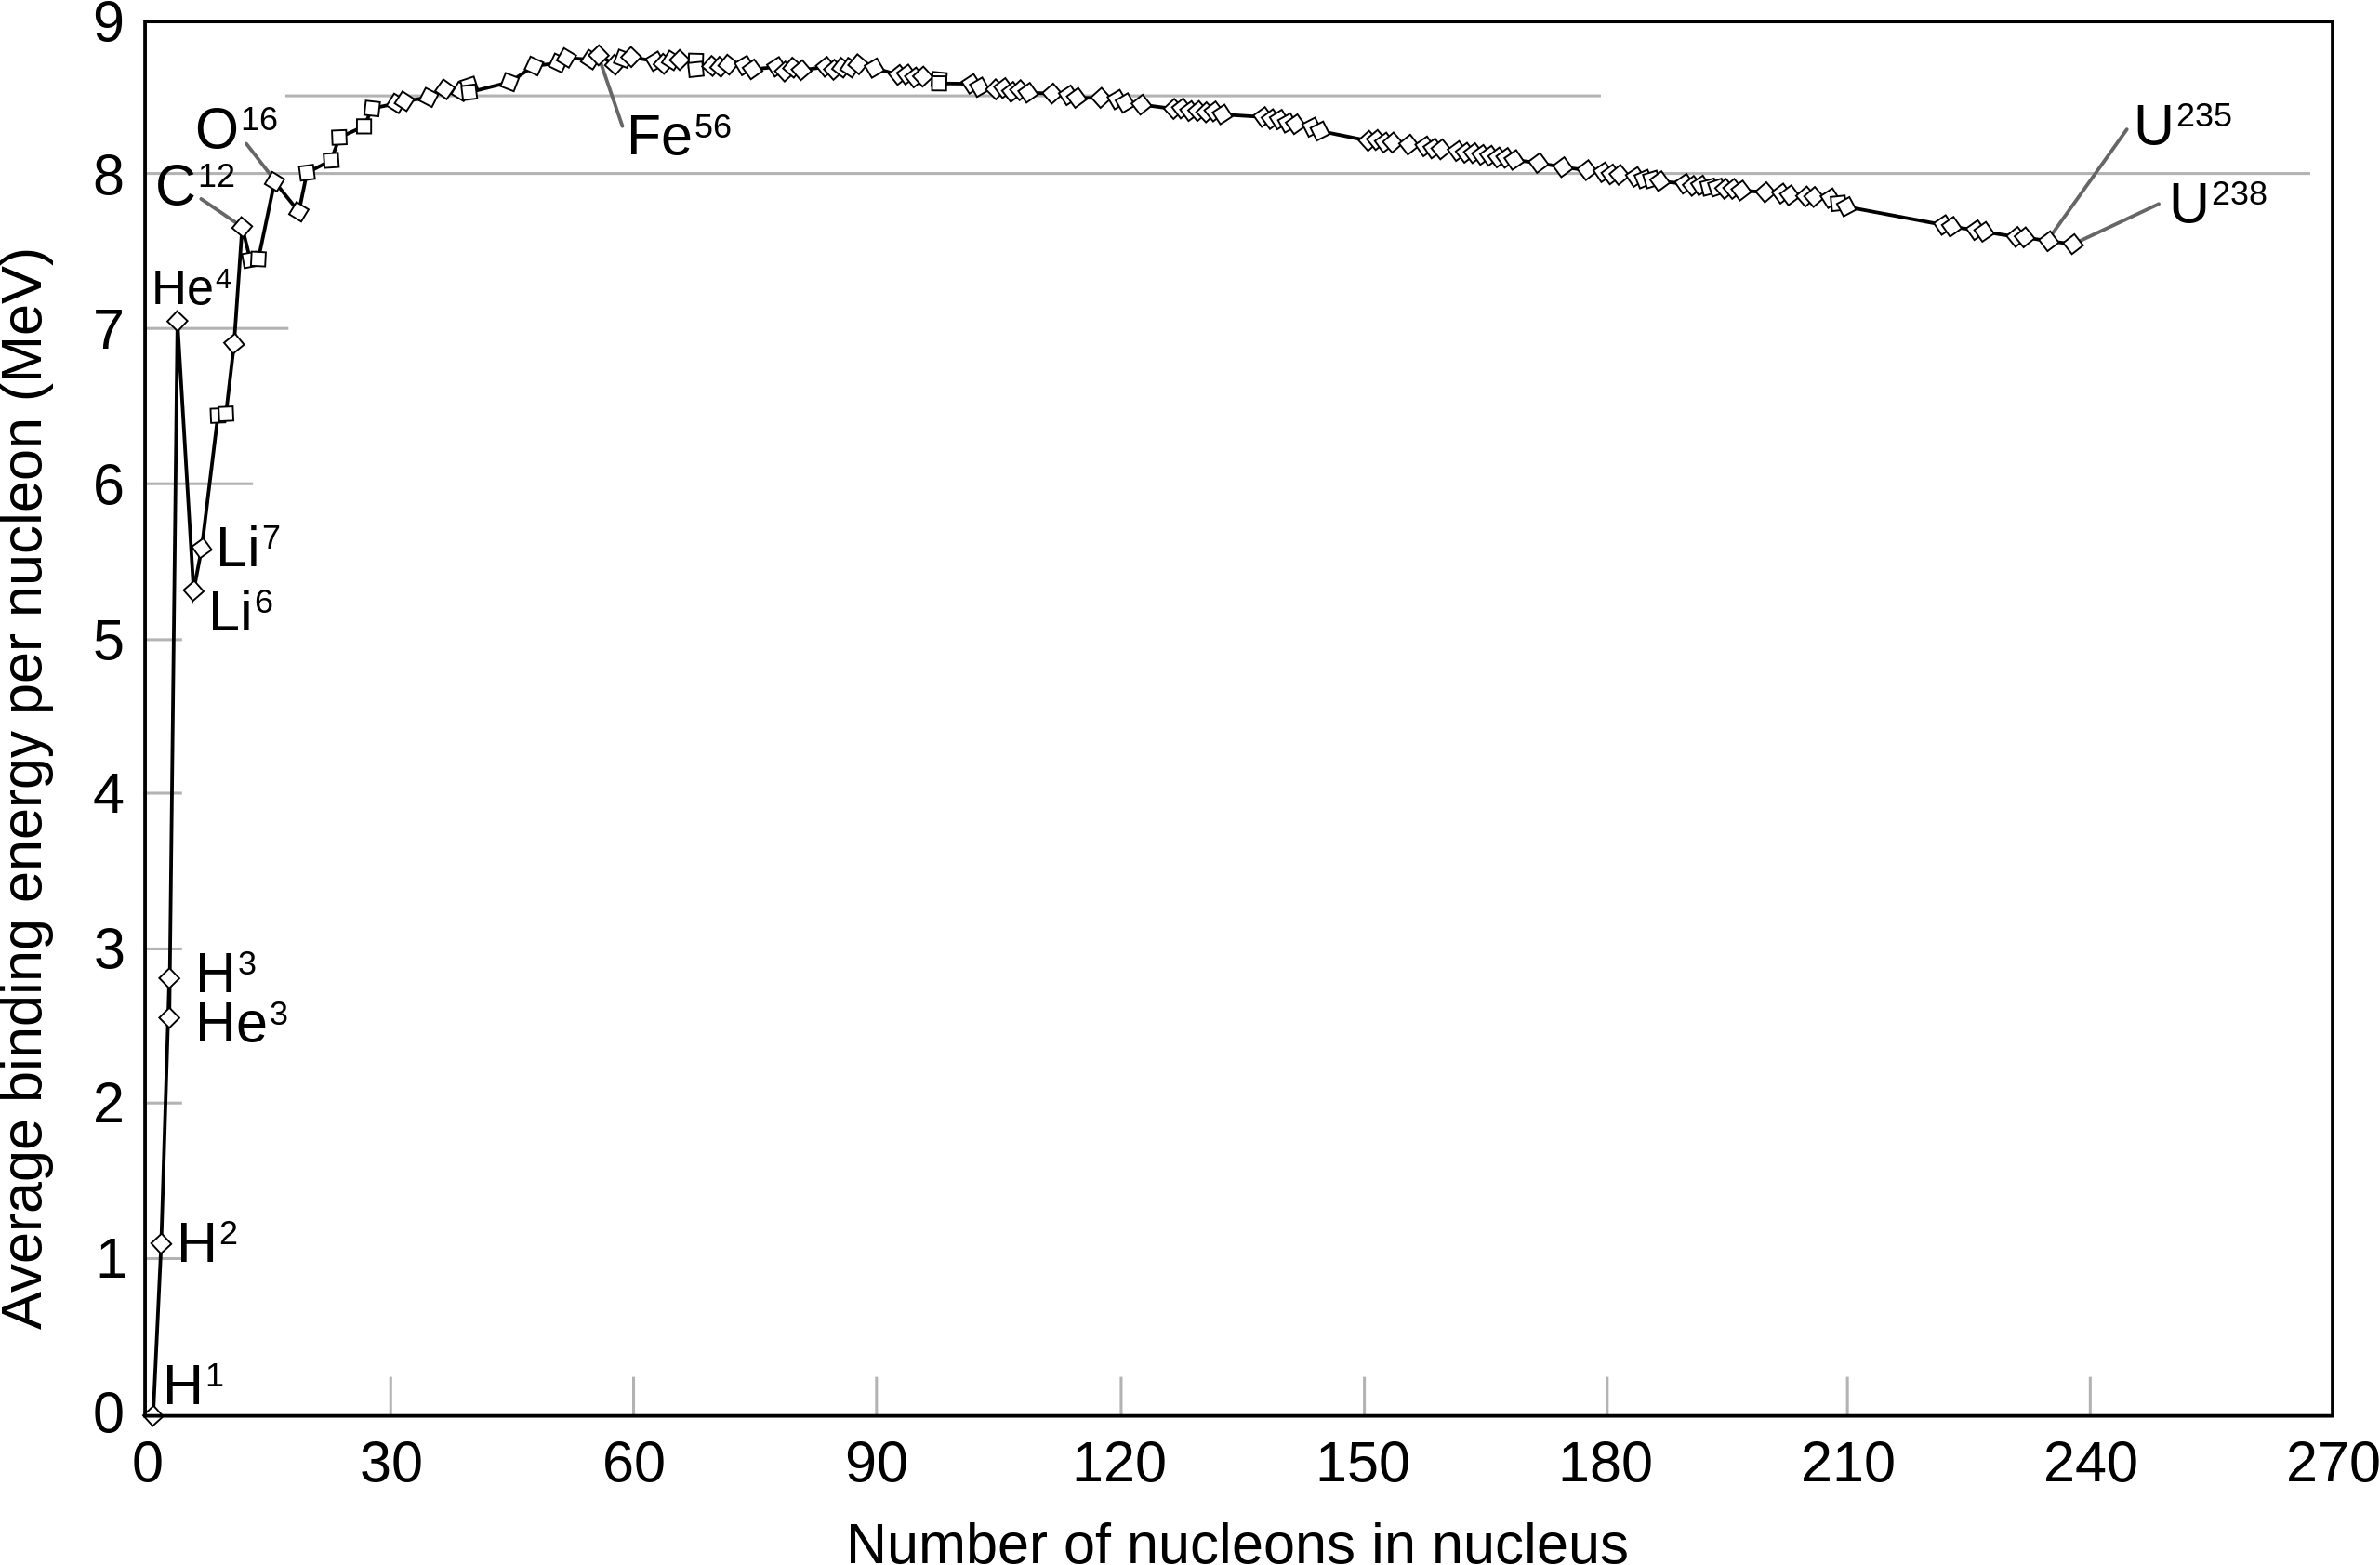
\includegraphics[width=0.5\textwidth]{img/nuclei.png}
    \caption{Andamento dell'energia media di legame per nucleone.}
    \label{fig:nuclei}
\end{figure}
Per far sì che avvenga il processo di fusione, i due protoni (o in generale i reagenti) devono vincere la repulsione coloumbiana, visualizzabile come una barriera di potenziale con legge $z_1 z_2 e^2 / r$, e raggiungere la distanza $r_0$ oltre la quale si ha una buca di potenziale ($0 < r < r_0$). Il valore del potenziale coulombiano a distanza $r_0$ lo chiameremo $B$ e per $r_0$ utilizzeremo una nota approssimazione del raggio nucleare, al di sotto della quale i reagenti possono interagire tramite interazione forte
\begin{gather*}
    B = \frac{z_1 z_2 e^2}{r_0},\\
    r_0 = A^{\frac{1}{3}}1\,\textup{fm}.
\end{gather*}
Se conosciamo l'energia cinetica dei protoni all'interno del sole possiamo determinare se i due protoni che si scontrano riescono a passare la barriera di potenziale o meno. Per fare dei conti numerici nel nostro caso basterebbe sostituire $z_1 = z_2 = A = 1$, otteniamo che $B = 1.5\,\textup{MeV}$. Vorremmo dunque ottenere l'energia cinetica dei protoni all'interno del sole. Per la precisione siamo interessati alla distribuzione in energia dei protoni all'interno del sole, che possiamo considerare distribuiti come una Maxwell-Boltzman
\begin{equation}
    f(E) \varpropto \sqrt{E} e^{-\frac{E}{kT}}\frac{1}{(kT)^{3/2}},\label{eq:maxwellbolz}
\end{equation}
ci interessa quindi ottenere una stima della temperatura all'interno del sole. L'idea da seguire è quella di imporre l'equilibrio idrostatico al sole, tra pressione del gas contenuto del sole e forza di attrazione gravitazionale del gas. Consideriamo un'area $\der S$ su di un guscio sferico del sole con raggio $r$ e spessore $\der r$
\begin{equation*}
    \begin{split}
        \frac{G m(r)\rho(r)\der S \der r}{r^2} & = \bigl(P(r) - P(r+\der r)\bigr)\der S\\
                                               & = -\frac{\der P}{\der r} \der r \der S,
    \end{split}
\end{equation*}
moltiplicando e dividendo il primo membro per $4\pi r^2$, possiamo aggiustare l'equazione come segue
\begin{equation}
    \frac{\der P}{\der m} = - \frac{Gm}{4\pi r^4}.
    \label{eq:sole1}
\end{equation}
Facciamo adesso una approssimazione al primo membro e assumiamo che la derivata sia costante, possiamo dunque sostituire il primo membro con il termine $\frac{P_\textup{c}}{M_\odot}$.
\begin{definition}
    Ciascuna grandezza relativa al sole viene sempre indicata con il pedice $\odot$. Ad esempio, riportiamo a scopo informativo i seguenti valori
    \begin{gather*}
        M_\odot = 2 \times 10^{30}\,\textup{kg},\\
        R_\odot = 0.7 \times 10^{9} \,\textup{m}.
    \end{gather*}
\end{definition}
Per approssimare il secondo membro di Eq.(\ref{eq:sole1}) possiamo supporre che in un volume corrispondente a metà del raggio sia contenuta metà della massa del sole. Dunque riscriviamo Eq.(\ref{eq:sole1}) come
\begin{equation}
    P_\textup{c} = \frac{G M_\odot^2}{R_\odot^4}\frac{2}{\pi}.
    \label{eq:pressione_sole}
\end{equation}
Dobbiamo dunque scrivere una equazione di stato per il gas contenuto nel sole, volendo correlare la pressione alla temperatura
\begin{equation*}
    PV = nkT = \sum_i n_i(Z_i + 1)kT,
\end{equation*}
dove al secondo passaggio abbiamo esplicitato le diverse specie che compongono il gas, ovvero protoni e elettroni. Con semplici considerazioni, possiamo riscrivere $n_i$ come seguente
\begin{equation*}
    n_i = \frac{\rho_i V N_\textup{A}}{A_i} = \frac{\rho_i}{\rho}\frac{N_\textup{A}}{A_i} \equiv x_i \frac{N_\textup{A}}{A_i}.
\end{equation*}
Sostituiamo dunque $n_i$ come ricavato adesso nella equazione di stato del gas e otteniamo 
\begin{equation}
    PV = \sum_i \frac{x_i (1 + Z_i)}{A_i}N_\textup{A} k T = \overline{n}\mathcal{R}T,
    \label{eq:pressione_sole2}
\end{equation}
dove $\mathcal{R} = N_\textup{A}k$ è la costante dei gas perfetti, $\overline{n}$ è il numero medio di moli per nucleone. Nel caso di una singola specie (di protoni) otteniamo $\overline{n} = 2$. Mettiamo dunque insieme Eq.(\ref{eq:pressione_sole}) e Eq.(\ref{eq:pressione_sole2}) nella quale sostituiamo $V$ con $1 / \rho_c$. Inoltre anticipiamo che maggioreremo il fattore $1 / \rho_c$ con il reciproco della pressione media $(\frac{4}{3} \pi R_\odot ^3) / M_\odot$. Otteniamo la seguente espressione per la temperatura al centro del sole
\begin{equation*}
    T_\textup{c} \leq \frac{4}{3}\frac{GM_\odot}{\mathcal{R}R_\odot} \simeq 3 \times 10^{7} \, ^\circ \textup{K}.
\end{equation*}
Possiamo dunque ricavare l'energia cinetica media delle particelle all'interno del sole1
\begin{equation*}
    E_\textup{kin} = \frac{3\times 10^7\,\textup{°K}}{1.2\times 10^4 \,\textup{eV}} \simeq 2.5\,\textup{keV}.
\end{equation*}
Considerando che la distribuzione di probabilità vista prima dipendeva da $e^{-E/kT}$ otteniamo che questo fattore vale circa $e^{-1.5\,\textup{MeV} / 2.5\,\textup{keV}}$, ovvero un fattore $\sim e^{-1000} \sim 10^{-400}$, questa ricordiamo essere la probabilità di attraversare la barriera coulombiana. Possiamo ottenere una stima di quanti nucleoni fondono semplicemente moltiplicando il numero ottenuto per il numero totale di nucleoni $N_\textup{N} \simeq M_\odot N_\textup{A} \simeq 1.2 \times 10^{57}$, il numero di nucleoni che fondono rimane comunque circa $0$. L'unica maniera che abbiamo di vedere un processo di fusione dunque è quello di considerare l'attraversamento della barriera per effetto tunnel
\begin{equation*}
    \Pr(\textup{effetto tunnel}) = \exp \biggl( \displaystyle\int_{r_0}^{r_1} \sqrt{\frac{2m}{\hslash ^2}\bigl( V(r) - \overline{E} \bigr)} \der r \biggr),
\end{equation*}
risolviamo dunque l'integrale come seguente
\begin{equation*}
    \begin{split}
        \displaystyle\int_{r_0}^{r_1} \sqrt{\frac{2m}{\hslash ^2}\bigl( V(r) - \overline{E} \bigr)} \der r & = \sqrt{\frac{2m}{\hslash ^2}z_1 z_2 e^2} \int_{r_0}^{r_1} sqrt{\frac{1}{r_0} - \frac{1}{r_1}} \der r \\
        & = (\dots) \frac{1}{\sqrt{r_1}} \int_{r_0}^{r_1} \sqrt{\frac{r_1}{r_0} - 1} \frac{\der r}{r_1} r_1 \\
        & = (\dots) \sqrt{r_1} \int_{r_0 / r_1}^{1} \sqrt{\frac{1}{x} - 1} \der x = (\dots) \sqrt{r_1} \frac{\pi}{2},
    \end{split}
\end{equation*}
dove per risolvere l'ultimo integrale abbiamo approssimato l'estremo inferiore come seguente
\begin{equation*}
    \begin{cases}
        B = \frac{z_1 z_2 e^2}{r_0} \\
        \overline{E} = \frac{z_1 z_2 e^2}{r_1} 
    \end{cases}
    \Rightarrow \frac{r_0}{r_1} = \frac{\overline{E}}{B} \simeq 0.
\end{equation*}
Possiamo dunque scrivere la probabilità di attraversamento della barriera per effetto tunnel come seguente
\begin{equation}
    \Pr (\textup{effetto tunnel}) = \exp \biggl( -\pi \sqrt{\frac{2m}{\hslash^2} \frac{(z_1 z_2 e^2)^2}{\overline{E}}}\biggr) \equiv e^{-\sqrt{\frac{E_\textup{G}}{\overline{E}}}}.\label{eq:gamow} 
\end{equation}
\begin{definition}[Energia di Gamow]
    Il termine $E_\textup{G}$ che compare in Eq.(\ref{eq:gamow}) viene chiamata \emph{energia di Gamow}
    \begin{equation*}
        E_\textup{G} = \frac{2m_\textup{r}\pi^2}{\hslash^2}(z_1 z_2 e^2)^2,
    \end{equation*}
    dove $m_\textup{r}$ è la massa ridotta delle due particelle con rispettivamente $z_1$ e $z_2$ unità di carica.
\end{definition}
Nel caso di protone-protone $E_\textup{G}$ vale circa $600\,\textup{keV}$. Considerando il valore prima ottenuto per l'energia media all'interno del sole $\sim 1 \,\textup{keV}$, otteniamo che la nuova probabilità di attraversamento della barriera vale circa $10^{-10}$, molto maggiore con il $10^{-400}$ di prima e sicuramente dà un numero di protoni che fondono sicuramente diverso da zero, dovendo moltiplicare per $10^{57}$ nucleoni.

Vogliamo adesso capire come misurare i neutrini provenienti dal sole e quanti aspettarsene. Scriviamo la sezione d'urto
\begin{equation*}
    \frac{\der N}{\der t \der V} = \frac{n(r)^2}{2} \sigma v_\textup{R},
\end{equation*}
dove $n(r)^2/2$ è un fattore che tiene di conto che proiettili e bersagli sono entrambi protoni, e il fattore 2 tiene di conto dell'identicità di queste due specie, $v_\textup{R}$ è la velocità relativa tra proiettile e bersaglio, $\sigma$ è la sezione d'urto per il processo di fusione. Notare che $n = n(r)$ poichè la densità di particelle sarà in generale una funzione del raggio, ci aspettiamo in particolare che la maggior parte delle particelle si trovi al centro del sole. Dunque vogliamo ricavare il rate di fusione, e successivamente di produzione di neutrini, al centro del sole. Se consideriamo $b$ il parametro d'impatto per il processo di fusione, dobbiamo richiedere che $b$ sia comparabile con il raggio nucleare medio affinchè il processo avvenga. Da questa considerazione proviamo a ricavare la sezione d'urto. Consideriamo il momento angolare
\begin{equation*}
    pb = l\hslash \Rightarrow b = l \frac{\hslash}{p},
\end{equation*}
per ottenere una stima della sezione d'urto \emph{geometrica} devo sommare su tutti i possibili momenti angolari
\begin{equation*}
    \sigma_\textup{G} = \pi \sum_l\bigl[ b^2(l+1) - b^2(l) \bigr] = \pi \biggl(\frac{\hslash}{p}\biggr)^2 \sum_l \bigl[ (l+1)^2 - l^2 \bigr] = \pi \biggl(\frac{\hslash}{p}\biggr)\sum_l[2l + 1].
\end{equation*}
La sommatoria dovrebbe andare da $0$ a $\infty$, ma siccome deve valere $b \leq r_0$, dobbiamo rispettrare la condizione $l \leq r_0 p /\hslash$. Possiamo in effetti dare una stima del termine a destra della disuguaglianza e otteniamo che $l \leq 10^{-2}$, conta cioè unicamente l'onda S. Aggiustando la sezione d'urto geometrica per proiettili di natura ondulatoria, si ottiene che 
\begin{equation*}
    \sigma_\textup{G} = \frac{4\pi \hslash^2}{2m \overline{E}} \sin2 \delta_0 (E) = \frac{S(\overline{E})}{\overline{E}}.
\end{equation*}
Il numeratore dell'ultima espressione viene anche chiamato \emph{fattore astrofisico}. Dunque adesso possiamo scrivere che
\begin{equation*}
    \frac{\der N}{\der t \der V} \varpropto n^2(r) \frac{S(E)}{E} e^{-\sqrt{E_\textup{G} / E}}\sqrt{E},
\end{equation*}
se adesso moltiplichiamo per la distribuzione di Maxwell-Boltzman Eq.(\ref{eq:maxwellbolz}), possiamo fare una media sull'energia
\begin{equation*}
    \begin{split}
        \frac{\der N}{\der t \der V} & \varpropto \int_0^\infty n^2(r) \frac{S(E)}{E} e^{-\sqrt{E_\textup{G} / E}}\sqrt{E}\sqrt{E} e^{-\frac{E}{kT}}\frac{1}{(kT)^{3/2}} \der E \\
        & \varpropto \frac{n^2}{(kT)^3}\int_0^\infty S(E) e^{-\biggl(\sqrt{\frac{E_\textup{G}}{E}} + \frac{E}{kT}\biggr)} \der E
    \end{split}
\end{equation*}
Il fattore astrofisico dipende in particolare dal tipo di nuclei coinvolti, che possono dar vita ad eventi di risonanza. Se assumiamo però che $S(E)$ vari poco possiamo semplificare i calcoli e risolvere l'integrale. L'argomento dell'esponenziale tra parentesi è composto da un termine lineare e uno iperbolico in $E$, dunque esiste una regione di valori intermedi di energia tra questi due regimi in cui l'argomento tra parentesi varrà meno. In questa stessa regione la funzione integranda vale il suo massimo valore (per via del segno negativo nell'esponenziale). Questo picco che raggiunge la funzione integranda si chiama \emph{picco di Gamow} (indichiamola con $E_0$), se questo è abbastanza stretto e se $S(E)$ non ha effetti di risonanza posso approssimare $S = S(E_0)$. Successivamente dobbiamo approssimare (al secondo ordine) la funzone seguente
\begin{equation*}
    -f(E) \equiv \sqrt{\frac{E_\textup{G}}{E}} + \frac{E}{kT},
\end{equation*}
studiando la derivata prima possiamo identificare $E_0$ come il suo punto di minimo. La posizione del picco di Gamow risulta essere
\begin{equation*}
    E_0 = \sqrt[3]{E_\textup{G}}\biggl( \frac{kT}{2} \biggr)^{2/3}
\end{equation*}
dunque
\begin{equation*}
    -f(E) = \frac{3E_0}{kT} \equiv \tau \Rightarrow \tau = 3 \sqrt[3]{\frac{E_\textup{G}}{4kT}} \simeq 12,
\end{equation*}
dove abbiamo introdotto la notazione della variabile $\tau$ e abbiamo calcolato il valore approssimato per il caso di protone-protone. Portiamo avanti i calcoli e otteniamo
\begin{equation*}
    -f(E_0)'' = \frac{3}{4}\sqrt{E_\textup{G}} E_0^{-\frac{5}{2}} = \frac{\tau}{2E_0^2},
\end{equation*}
la funzione $f$ in un intorno del punto $E_0$ è approssimabile come seguente
\begin{equation*}
    f(E) \simeq -\tau -\frac{\tau}{4E_0^2}(E - E_0)^2,
\end{equation*}
quindi l'integrale iniziale da valutare che mi dà il rate è 
\begin{equation*}
    R \varpropto \frac{n^2}{(kT)^{3/2}} \int_0^\infty e^{-\tau} e^{-\frac{\tau}{4E_0^2}(E-E_0)^2}\der E,
\end{equation*}
eseguiamo il seguente cambio di variabile
\begin{gather*}
    \frac{\sqrt{\tau}}{2E_0}(E-E_0) = \xi \\
    \der \xi = \frac{\sqrt{\tau}}{2E_0}\der E,
\end{gather*}
riprendendo l'integrale abbiamo
\begin{equation*}
    R \varpropto \frac{n^2}{(kT)^{3/2}} e^{-\tau} \frac{2E_0}{\sqrt{\tau}}\int_{-\sqrt{\tau}/2}^{\infty} e^{-\xi^2} \der \xi.
\end{equation*}
Approssimando l'integrale tra $-\infty$ a $+\infty$, possiamo riscrivere l'espressione del rate $R$
\begin{equation*}
    R \varpropto \frac{n^2}{(kT)^{3/2}}e^{-\tau}\frac{E_0}{\sqrt{\tau}},
\end{equation*}
esplicitiamo la dipendenza da $\tau$, osserviamo che la potenza rimanente è $\tau^2$
\begin{equation*}
    R \varpropto \tau^2 e^{-\tau},
\end{equation*}
questa in effetti ci dice la dipendenza dalla temperatura all'interno del sole per il rate di fusione, quindi per il rate di produzione di neutrini. Se vogliamo esprimere questa dipendenza come $T^{\nu}$, ne facciamo il logaritmo
\begin{equation*}
    \log R = \textup{cost} + \nu \log T \Rightarrow \nu = \frac{\partial \log R}{\partial \log T},
\end{equation*}
per quanto abbiamo scritto prima vale anche
\begin{equation*}
    \log R = \textup{cost} + 2 \log \tau - \tau
\end{equation*}
quindi
\begin{equation*}
    \frac{\partial \log R}{\partial \log T} = 2 \frac{\partial \log \tau}{\partial \log T} - \frac{\partial \tau}{\partial \log T} = (2 - \tau) \frac{\partial \log \tau}{\partial \log T},
\end{equation*}
dato che $\tau \varpropto T^{-1/3}$ e quindi $\log \tau = \textup{cost} - \frac{1}{3} \log T$, mettendo tutto insieme otteniamo che
\begin{equation*}
    \nu = \frac{\tau}{3} - \frac{2}{3},
\end{equation*}
nel caso di protone-protone sappiamo che $\tau = 12$, quindi $\nu \sim 3.3$. Volendo stimare la precisione con cui misuriamo il rate possiamo scrivere
\begin{equation*}
    \frac{\Delta R}{R} = \nu \frac{\Delta T}{T},
\end{equation*}
la dipendenza lineare da $\nu$ fa sì che, data la crescenza di $\nu$ per nuclei più pesanti, l'incertezza sul rate di neutrini sia maggiore.


%----------------------------------------------------------------------------------------
% 	APPENDICI
\begin{appendices} %---------------------------------------------------------------------
\renewcommand{\chaptername}{Appendice}

	\chapterimage{img/SuperKK.jpg} % Chapter heading image
\chapterspaceabove{6.75cm} % Whitespace from the top of the page to the chapter title on chapter pages
\chapterspacebelow{7.25cm} % Amount of vertical whitespace from the top margin to the start of the text on chapter pages

%------------------------------------------------

\chapter{Fluidodinamica}\label{chap:app1}

In questa appendice ripasseremo alcuni concetti utili per il corso, riguardo alla fluidodinamica.

Consideriamo le quantità principali che ci aiutano a modellizzare e descrivere il sistema:
\begin{gather*}
    \rho = \rho(x, y, z, t),\\
    \vec{v} = \vec{v}(x, y, z, t).
\end{gather*}

\section{Prima equazione di continuità}
Consideriamo un fluido con una certa densità $\rho$, una velocità $\vec{v}$, e ci interroghiamo sulla quantità di fluido che nell'unità di tempo passa per una certa superficie orientata $\der \vec{S}$
\begin{equation*}
    \rho v \cos \theta \der S = \rho \frac{\der V}{\der t} = \rho \vec{v}\cdot \hat{n} \der S,
\end{equation*}
addesso integriamo questa espressione su una superficie e applichiamo successivamente il teorema della divergenza per ottenere
\begin{equation}
    \int_V \biggl[ \frac{\partial \rho}{\partial t} - \vec{\nabla} \cdot (\rho \vec{v}) \biggr] \der V = 0. \label{eq:continuita1}
\end{equation}
Eq.(\ref{eq:continuita1}) impone una legge di conservazione (equazione di continuità) tra la variazione di materia all'interno di un volume e il flusso della stessa materia attraverso la superficie del volume.

\section{Seconda equazione di continuità}
Nelle stesse condizioni di prima, possiamo affermare che il fluido esercita una pressione sulla superficie $S$ pari a $p \der S$, la forza che agisce sulla superficie è dunque 
\begin{equation*}
    \vec{F} = - \int_S p\der \vec{S}. 
\end{equation*}
Vogliamo scrivere questa relazione in modo puntuale, come prima. Possiamo utilizzare nuovamente il teorema della divergenza su ciascuna delle componenti di una funzione vettoriale $\vec{u}$ che posso scegliere in maniera arbitraria fatta come $\vec{u} = (p, p, p)$. Otteniamo dunque
\begin{equation*}
    \vec{F} = - \int_S p\der \vec{S} = - \int_V \vec{\nabla} p \der V.
\end{equation*}
Adesso vogliamo ricavare la legge di conservazione dell'impulso, per farlo partiamo considerando la quantità di materia con una certa velocità $v_i$ che esce dal volumne nel tempo $\der t$ e ci chiediamo quanto valga la variazione di impulso che fuoriesce dal volume $V$ nello stesso intervallo di tempo
\begin{equation*}
    \int_S \rho v_i \vec{v} \cdot \hat{n} \der S = \frac{\partial}{\partial t} \int_V (\rho v_i) \der V,
\end{equation*}
vogliamo però un integrale di volume, dunque sfruttiamo la relazione di prima e otteniamo
\begin{equation*}
    \frac{\partial}{\partial t} \int_V (\rho v_i) \der V = - \int_V \sum_j \partial_j (\rho v_i v_j) \der V,
\end{equation*}
raccogliendo i vari termini otteniamo alla finale
\begin{equation*}
    \int_V \biggl[ \frac{\partial}{\partial t} (\rho v_i) + \sum_j\frac{\partial}{\partial x_j}(\rho v_i v_j) \biggr] \der V = 0.
\end{equation*}
Possiamo adesso aggiungere il contributo della forza, ovvero il gradiente della pressione
\begin{equation}
    \frac{\partial}{\partial t} (\rho v_i) + \sum_j\frac{\partial}{\partial x_j}(\rho v_i v_j) = - \frac{\partial p}{\partial x_i},\label{eq:rhovivj}
\end{equation}
questa è la conservazione dell'impulso per un fluido. Per scriverla meglio possiamo riarrangiare i termini a questa maniera
\begin{equation}
    \frac{\partial}{\partial t} (\rho v_i) = - \frac{\partial}{\partial x_j}(P\delta_{ij} + \rho v_i v_j),
\end{equation}
dove al secondo membro abbiamo ottenuto un tensore. Espandendo le derivate al primo menbro in Eq.(\ref{eq:rhovivj}), raccogliendo $v_i$ e semplificando un termine che risulta uguale alla prima equazione di continuità Eq.(\ref{eq:continuita1}), scriviamo il risultato ottenuto in forma vettoriale
\begin{equation}
    \frac{\partial \vec{v}}{\partial t} + (\vec{v} \cdot \vec{\nabla}) \vec{v} = - \frac{1}{\rho} \vec{\nabla} p. \label{eq:eulero}
\end{equation}
Eq.(\ref{eq:eulero}) si chiama \emph{equazione di Eulero}.

\section{Conservazione dell'energia}
Consideriamo tutte le funzione, come velocità e pressione, per volumi di massa unitaria, cioè $\rho V = 1$. Adottiamo $s \equiv S / M$, cioè l'entropia per unità di massa. Trascuriamo inoltre tutti i fenomeni che comportano una non conservazione dell'energia meccanica, ad esempio la viscosità e la conducibilità termica, come se non ci fosse un trasferimento di calore da una porzione all'altra del volume. Quindi stiamo imponendo che $\der S = 0$. Scrivendolo in funzione delle derivate parziali
\begin{equation*}
    \frac{\der s}{\der t} = \frac{\partial s}{\partial t} + \sum_{i = 1}^3 \frac{\partial s}{\partial x_i} v_i = 0.
\end{equation*}
Vogliamo scrivere la stessa cosa per l'energia. Prendiamo un volume di massa unitario, quindi di energia cinetica $\frac{1}{2}\rho v^2$, insieme a questa devo considerare anche l'energia interna del fluido $U / V = \frac{U}{M} \frac{M}{V} \equiv \epsilon \rho$. Vogliamo vedere quanta di questa energia totale fluisce attraverso la superficie che delimita il volume che sto considerando. Faremo il conto nel caso unidimensionale, utilizzando dove necessario le prime due equazioni di continuità. Deriviamo quindi rispetto al tempo l'energia totale e otteniamo
\begin{equation}
    \frac{\partial}{\partial t}\biggl( \frac{1}{2}\rho v^2 + \epsilon \rho \biggr) = \frac{1}{2} \frac{\partial \rho}{\partial t} v^2 + \frac{1}{2}\rho \frac{\partial v^2}{\partial t} + \frac{\partial \epsilon}{\partial t} \rho + \epsilon \frac{\partial \rho}{\partial t}.\label{eq:continuita3}
\end{equation}
Osserviamo che i primi due termini e il quarto termine nel secondo membro possiamo riscriverli utilizzando appunto Eq.(\ref{eq:continuita1}) e Eq.(\ref{eq:eulero}). Per il terzo termine utilizziamo un noto principio della termodinamica
\begin{equation*}
    \der \epsilon = T \der s - p \der V = T \der s - p \der \biggl( \frac{1}{\rho} \biggr) = T \der s + p \biggl( \frac{\der \rho}{\rho^2} \biggr),
\end{equation*}
facciamo la derivata parziale rispetto al tempo e otteniamo 
\begin{equation*}
    \frac{\partial \epsilon}{\partial t} = T \frac{\partial s}{\partial t} + \frac{p}{\rho^2} \biggl( \frac{\partial \rho}{\partial t} \biggr).
\end{equation*}
Con questo risultato possiamo riscrivere il seguente termine 
\begin{equation*}
    \begin{split}
        \rho \frac{\partial \epsilon}{\partial t} + \epsilon \frac{\partial \rho}{\partial t} & = - \rho Tv \frac{\partial s}{\partial x} + \frac{p}{\rho} \frac{\partial \rho}{\partial t} + \epsilon \frac{\partial \rho}{\partial t}\\
                                                                                              & = - \rho Tv \frac{\partial s}{\partial x} + \frac{\partial \rho}{\partial t} (\epsilon + pV).
    \end{split}
\end{equation*}
L'ultimo termine tra parentesi prende il nome di \emph{entalpia}. Per l'entalpia vale la seguente relazione
\begin{equation*}
    \der h = \der (\epsilon + pV) = T \der s + V \der p \Longrightarrow T \der s = \der h - V \der p,
\end{equation*}
posso utilizzare l'ultima uguaglianza per riscrivere il seguente termine
\begin{equation*}
    - \rho T v \frac{\partial s}{\partial x} = - \rho v \frac{\partial h}{\partial x} + v \frac{\partial p}{\partial x}.
\end{equation*}
Dunque 
\begin{equation*}
    \rho \frac{\partial \epsilon}{\partial t} + \epsilon \frac{\partial \rho}{\partial t} = \frac{\partial \rho}{\partial t} h - \rho v \frac{\partial h}{\partial x} + v \frac{\partial p}{\partial x},
\end{equation*}
siamo riusciti a riscrivere gli ultimi due termini di Eq.(\ref{eq:continuita3}). Possiamo dunque adesso riscrivere Eq.(\ref{eq:continuita3}) facendo le varie sostituzioni discusse fino ad ora al secondo membro ed otteniere una nuova equazione che poi integreremo sul volume
\begin{gather*}
    \frac{\partial}{\partial t}\biggl( \frac{1}{2}\rho v^2 + \epsilon \rho \biggr) = - \frac{\partial}{\partial x}\biggl( \rho v \biggl( \frac{1}{2} v^2 + h \biggr) \biggr), \\
    \begin{align}
        \int_V \frac{\partial}{\partial t}\biggl( \frac{1}{2}\rho v^2 + \epsilon \rho \biggr) \der V & = - \int_V \vec{\nabla} \cdot \biggl[ \rho \vec{v} \biggl( \frac{1}{2} v^2 + h \biggr) \biggr] \der V\\
                                                                                                     & = - \int_S \rho \vec{v} \biggl( \frac{1}{2} v^2 + h \biggr) \cdot \der S.
    \end{align}
\end{gather*}
Chiamiamo $\vec{J}$ il vettore densità di flusso di energia attraverso una superficie, questo è dato dal secondo membro dell'equazione scritta prima
\begin{equation*}
    \vec{J} = \rho \vec{v} \biggl( \frac{1}{2} v^2 + \epsilon + \frac{p}{\rho} \biggr),
\end{equation*}
se otteniamo che la derivata rispetto al tempo è nulla, abbiamo la conservazione della corrente.

\begin{example}[Piccole perturbazioni di un fluido]
    Consideriamo, nel caso adiabatico, piccole perturbazioni di un fluido. Se scriviamo $p = p_0 + p'$ con $p' \ll p_0$ la perturbazione, analogamente $\rho = \rho_0 + \rho '$ con $\rho' \ll \rho_0$. Notiamo che se assumiamo adiabaticità l'energia è conservata. Nelle approssimazioni assunte in questo esempio vogliamo riscrivere le Eq.(\ref{eq:continuita1}) e Eq.(\ref{eq:continuita3}) trascurando gli infinitesimi di ordine superiore al primo. Quindi otteniamo
    \begin{equation}
        \begin{cases}
        \displaystyle\frac{\partial \rho'}{\partial t} + \rho_0 \vec{\nabla} \cdot \vec{v}\\
        \displaystyle\frac{\partial \vec{v}}{\partial t} = - \frac{\vec{\nabla}p'}{\rho_0\bigl( 1 + \frac{\rho'}{\rho_0} \bigr)} \simeq - \frac{\vec{\nabla} p'}{\rho_0}
        \end{cases}.\label{eq:fluidoadiab}
    \end{equation}
    Abbiamo scritto due equazioni con l'obiettivo di ricavare le tre variabili $\vec{v}$, $\rho'$ e $p'$. Imponiamo di sapere una funzione di stato che lega $p$ e $\rho$ per avere una terza equazione $p = f(\rho)$, dunque imponendo anche $p' = \bigl(\partial_\rho f(\rho)\bigr)\bigr|_{\rho = \rho_0}\rho'$. Dunque possiamo scrivere nuovamente il sistema di Eq.(\ref{eq:fluidoadiab}) come seguente
    \begin{equation*}
        \begin{cases}
            \displaystyle\frac{1}{\bigl(\partial_\rho p\bigr)\bigr|_{\rho = \rho_0}} \frac{\partial p'}{\partial t} + \rho_0 \vec{\nabla} \cdot \vec{v} = 0\\
            \displaystyle\frac{\partial \vec{v}}{\partial t} = \frac{\vec{\nabla} p'}{\rho_0}
        \end{cases}.
    \end{equation*}
    Cerchiamo la soluzione della forma $\vec{v} = \vec{\nabla} \varphi$, sostituendo nella seconda equazione otteniamo
    \begin{equation*}
        p' = - \rho_0 \frac{\partial \varphi}{\partial t},
    \end{equation*}
    sostituendo nella prima equazione del sistema otteniamo che 
    \begin{equation}
        - \frac{1}{c_\textup{s}^2} \frac{\partial ^2 \varphi}{\partial t^2} + \nabla^2 \varphi = 0. \label{eq:fluidonda}
    \end{equation}
    Eq.(\ref{eq:fluidonda}) è la nota equazione d'onda, dove abbiamo sostituito a $\bigl( \partial_\rho p \bigr)\bigr|_{\rho = \rho_0}$ la quantità $c_\textup{s}^2$ che è la velocità di propagazione del suono nel mezzo. Come ben noto la soluzione è 
    \begin{equation*}
        \varphi = \alpha f_1(x - c_\textup{s}t) + \beta f_2(x + c_\textup{s}t).
    \end{equation*}
    Se consideriamo l'aria come gas perfetto, dunque affermando che $pV = \mu R T = n k_\textup{B} T = \mu N_\textup{A} k_\textup{B} T$, con $k_\textup{B} \sim \frac{1}{12000}\,\textup{eV}/\textup{°K}$. Nel caso di volume costante possiamo scrivere
    \begin{equation*}
        \der U = \der Q \Longrightarrow \mu c_\textup{v}\der T =\der U.
    \end{equation*}
    Per un gas di $n$ molecole con $g$ gradi di libertà sappiamo che $U = \frac{ng}{2}k_\textup{B}T$, possiamo ricavare che $c_\textup{v} = \frac{R}{2}g$. Nel caso a pressione costante abbiamo che 
    \begin{equation*}
        \der Q = \der U + p \der V \Longrightarrow \mu c_\textup{p} \der T = \mu c_\textup{v} \der T + \mu R \der T,
    \end{equation*}
    quindi ottenendo $c_\textup{p} = c_\textup{v} + R$
    \begin{definition}
        Definiamo $\gamma$ il rapporto $c_\textup{p} / c_\textup{v}$. Nel caso di gas monoatomico abbiamo che $g = 3$ e quindi $\gamma = 5/3$, nel caso di gas biatomico $\gamma = 7/5$. 
    \end{definition}
    Nel caso di trasformazioni adiabatiche sappiamo che $pV^\gamma = \textup{costante}$, dunque $p = c \rho^\gamma$. Dato che abbiamo detto che $c_\textup{s}^2 = \bigl( \partial_\rho p \bigr)\bigr|_{\rho = \rho_0}$, otteniamo che 
    \begin{equation*}
        c_\textup{s} = \sqrt[2]{\gamma pV}.
    \end{equation*}
    Se consideriamo ad esempio il caso dell'aria, modellizzandola come una miscela composta al $50\%$ di $\textup{O}_2$ e al $50\%$ di $\textup{N}_2$ si ottiene che $c_\textup{s} \simeq 340\,\textup{m}/\textup{s}$.
\end{example}


\end{appendices} %-----------------------------------------------------------------------

\end{document}